\chapter{Здаровыя звычкі}

\section{Звычкі як шкілет здароўя}

``Я займаюся здароўем, але нічога не атрымліваецца'',~--- мне рэгулярна даводзіцца чуць такія скаргі. І я часта бачу, што людзі шмат чытаюць пра здароўе, увесь час пра гэта кажуць, спрабуюць нешта рабіць, але не атрымліваюць вынікаў. Для іх займацца сваім здароўем цяжка~--- яны робяць усё, прымушаючы сябе, пачынаюць і кідаюць то правільнае харчаваньне, то заняткі спортам. Гадавыя абанементы ў~залу згараюць, а~хатнія трэнажоры становяцца вешалкамі для адзеньня. Ім быццам бы хочацца займацца, але першаснага імпульсу не хапае, і праз тыдзень-два ўсе добрыя пачынаньні глухнуць. А чым больш людзі сябе за гэта дакараюць, тым менш хочацца працягваць.

Вядома, такі бессыстэмны падыход павялічвае нездаволенасьць сабой. Так бывае, што людзі ўспрымаюць заняткі здароўем як нейкую моду, купляючы кілімок для ёгі, каштуючы супэрфуды, спампоўваючы ЗЛЖ-праграмы,~--- але тэарэтычны інтарэс не ўвасабляецца на практыцы. Толькі звычка дапамагае працягнуць рух, як казаў пісьменьнік Мішэль дэ Мантэнь: «Варта адрозьніваць душэўны парыў чалавека ад цьвёрдай і сталай звычкі».

\infobox{Усе мы гатовыя пачаць новае жыцьцё з~панядзелка, але наколькі нас хопіць? Часта мы закідваем свае пачынаньні і дакараем сябе за гэта, памяншаючы шанцы на другую спробу.}

Іншыя ж людзі менш ведаюць, менш гавораць і не выкладваюць матывавальныя фота ў~сацсетках, але рэгулярна, кожны дзень нешта робяць і клапоцяцца пра сябе. Вельмі часта такія рэгулярныя дзеяньні не зьяўляюцца асабістым дасягненьнем чалавека, яны маглі ўвайсьці ў~лад жыцьця з~бацькоўскай сям'і, несьвядома.

\emph{Навукоўцы заўважылі, што харчовыя патэрны, рэжым дня, звычка да спорту і догляду за сабой фармуюцца яшчэ ў~дзяцінстве. Не выпадкова Ф. Дастаеўскі прыкмеціў, што ``ўся другая палова чалавечага жыцьця складаецца звычайна з~адных толькі назапашаных у~першую палову звычак''.}

Мы верым у~сілу розуму, але паўсядзённым кіраўніком у~жыцьці зьяўляецца менавіта звычка. Паспрабуйце растлумачыць курцу, што курэньне шкоднае. Ён пагодзіцца, але не перастане курыць. Разуменьне праблемы, прызнаньне праблемы розумам зусім ня значыць, што гэта прывядзе да зьмены ладу жыцьця.

\textbf{Здаровую звычку }варта выбудоўваць на навуковай аснове, а~для гэтага трэба прайсьці пяць пасьлядоўных этапаў: веданьне, разуменьне, уменьне, навык, звычка.

\subsection*{Веданьне}

Атрымаць інфармацыю ў~сучасным сьвеце лёгка, але гэтак жа лёгка заблытацца ў~яе лішку. Часта людзі, якія прайшлі мае курсы, кажуць аб палягчэньні, калі яны пазбаўляюцца мноства псэўданавуковых тэорый і могуць сфакусавацца на сапраўды важных для здароўя рэчах. У папярэдніх разьдзелах выкладзена дастаткова ведаў для вядзеньня здаровага ладу жыцьця.

Парадокс: само па сабе веданьне аб тым, што шкодна, а~што карысна, не ўплывае на паводзіны. Дасьледаваньні паказваюць, што частата нездаровых паводзінаў у~падлеткаў павялічваецца па меры сталеньня, з~15 да 30 гадоў, незалежна ад ведаў аб яго рызыках. Многія людзі выказваюць намер весьці здаровы лад жыцьця, але ня робяць гэтага~--- так узьнікае разрыў намеру і дзеяньня. Дасьледаваньне паказала, што нават працяглае навучаньне дыябэтыкаў ня моцна паўплывала на іх лад жыцьця і біямаркеры (глікаваны гемаглабін, ліпідны профіль, вага), а~таксама рызыкі ўскладненьняў.

\emph{Ёсьць просты спосаб ацаніць, наколькі цэласная ваша псыхіка. Выпішаце на аркушы паперы ўсе рэчы, якія трэба рабіць, хочаце рабіць і якія робіце. Чым вышэйшы адсотак супадзеньня, тым лепш.}

Для захаваньня стабільнасьці псыхікі ёсьць цэлы набор абаронаў, якія дазваляюць нам нічога не рабіць з~праблемай. Тэрмін аназагназія, які азначае адсутнасьць крытычнай ацэнкі свайго стану,~--- ужываўся ў~мінулым для псыхічнай паталёгіі, але цяпер выкарыстоўваецца і для такіх паталёгій, як атлусьценьне, дыябэт, сардэчна-сасудзістыя захворваньні. Чалавек так «тлумачыць» праблемы з~вагой, памяцьцю і мысьленьнем: «я проста стаміўся», «пасьля 40 гэта норма», «у мяне стрэс», «з жыватом самавіты выгляд», «гэта мой выбар» і да т.~п. Людзі могуць выкарыстоўваць розныя інструмэнты абароны: пазьбяганьне, адмаўленьне, абсурдызацыю, гумар: «Ты памрэш!~--- Ха-ха, усе памруць». Зьмены пры хваробах ладу жыцьця звычайна такія плыўныя і незаўважныя, што чалавек да іх звыкае і пачынае лічыць сваёй ``нормай''. 

Адукацыя пацыентаў здаецца выхадам з~сытуацыі. Але калі празьмерна палохаць людзей наступствамі і небясьпекамі, то яны пачынаюць выкарыстоўваць нездаровыя копінг-стратэгіі і псыхічныя абароны, каб адысьці ад непрыемнай інфармацыі. Рацыянальна спрачацца з~такім пацыентам бессэнсоўна, вы толькі мацней пераканаеце яго ў~адваротным. Бо адмаўленьне сваёй праблемы для яго~--- гэта спосаб падтрыманьня ідэнтычнасьці. Таму патрэбныя не сухія веды, а~жывыя прыклады, эмацыйнае ўзьдзеяньне, уцягваньне ў~групы падтрымкі, паступовасьць.

\subsection*{Разуменьне}

Гэта наступная ступень на шляху да звычкі, калі атрыманыя веды трэба прыняць, спасьцігнуць іх сэнс, упусьціць у~сябе, уключыць гэтыя веды ў~сваю асабістую сыстэму ідэяў і ўяўленьняў. Інакш мы будзем, як папугі, прамаўляць бессэнсоўныя для сябе словы. Наш арганізм можа засвоіць бялкі, тлушчы і крухмалы, толькі расшчапіўшы іх да базавых амінакіслот, тлустых кіслот, монасахарыдаў і ў~такім выглядзе улучыўшы іх у~свае малекулы. Так і веды трэба перастрававаць, а~для гэтага важна старанна ``грызьці граніт навукі'' і мець добры апэтыт і цікаўнасьць.

\textbf{Разуменьне~--- гэта сапраўдны сэнсавы кантакт} зь веданьнем, калі мы бачым сувязь атрыманых ведаў са сваім жыцьцём і са сваімі каштоўнасьцямі. На маіх навучальных курсах я стараюся падвесьці вучняў да самастойнага разуменьня важнасьці ведаў, для гэтага мы разьбіраем тэмы здароўя на дастаткова глыбокім узроўні. Бо калі чалавек сам зразумеў, як гэта працуе, то гэта робіць атрыманае разуменьне асабістым дасягненьнем, сапраўдным азарэньнем, устойлівым і эфэктыўным~--- у~адрозьненьне ад вонкавай матывацыі. Вылучаюць разумовае і эмацыйнае азарэньні, якія дапамагаюць нам лепш разумець таксама і тое, што адбываецца з~намі. У гэтым разьдзеле вы знойдзеце шэраг практыкаваньняў, якія дапамогуць вам лепш зразумець сябе.

\subsection*{Уменьне}

Уменьне~--- гэта здольнасьць самастойна зрабіць пэўнае дзеяньне, пераход ад тэорыі і разуменьня да рэальнага дзеяньня пад усьвядомленым кантролем. Напрыклад, вы можаце разьвіць уменьне гатаваць, але яно патрабуе намаганьняў, калі важна памятаць і якія інгрэдыенты купіць, і колькі часу варыць, і калі пераварочваць.

Часта людзі не пераходзяць ад тэорыі да практыкі, бо пераскокваюць праз прыступку ўменьня.

\infobox{Важна навучыцца правільна выбіраць прадукты, правільна рэагаваць на стрэс, правільна бегаць~--- і лепш адразу вучыцца правільнаму, бо перавучвацца~--- нашмат складаней! Ня ўмееце гатаваць? Прайдзіце кулінарныя курсы! Няма тэхнікі сілавых практыкаваньняў? Навучыцеся ў~трэнэра! Няма добрай дыкцыі і баіцеся выступаць? Навучыцеся прамоўніцкаму майстэрству!}

\subsection*{Навык}

Гэта здольнасьць выконваць пэўныя дзеяньні, у~нашым выпадку~--- у~галіне здаровага ладу жыцьця,~--- якая ўзьнікла шляхам шматразовага паўтарэньня і ўсьвядомленага паляпшэньня. Навык паступова разьвіваецца і ўмацоўваецца па меры практыкі, пры гэтым зьмены часьцей за ўсё назапашваюцца неўпрыкмет.

Разьвіты навык~--- гэта калі мы можам нешта рабіць лёгка, правільна, з~задавальненьнем і карысьцю. Напрыклад, навык гатаваць, правільна прысядаць, спраўляцца з~голадам, расслабляцца, плянаваць, атрымліваць задавальненьне ад ежы. З практыкаю ўсьвядомленае дзеяньне, якое патрабуе кантролю і валявых намаганьняў, становіцца аўтаматычным і пераходзіць у~вобласьць працэдурнай памяці.

\subsection*{Звычка}

Звычка~--- гэта ўжо спосаб паводзінаў, патрэба паводзіць сябе пэўным чынам. Прытрымлівацца звычкі прыемна і лёгка, яна не расходуе шмат разумовых рэсурсаў. Уявіце сабе, што кожны чалавек~--- гэта кампутар, вы можаце ўсталяваць на яго розныя праграмы і правільна наладзіць іх. Хуткасьць працы будзе залежаць ня толькі ад самага жалеза, але й ад софту.

\subsection*{Шлях да здароўя}

\textbf{Шлях да здароўя можна ўявіць як лесьвіцу}, дзе кожная прыступка~--- гэта здаровая звычка. Чым больш у~вас звычак, тым вышэй вы падымаецеся і тым мацнейшае ваша здароўе. Найважнейшай часткай сваёй працы я лічу ня проста расказваць пра здароўе, а~дапамагаць людзям на практыцы ўкараняць здаровыя звычкі і дасягаць сваіх мэтаў. Важна не абвінавачваць людзей у~тым, што яны гультаі, а~шукаць, што спрацуе канкрэтна для гэтага чалавека. Бо які сэнс у~прызначэньнях і рэкамэндацыях, калі ваш пацыент іх усё роўна не выконвае?

Як той казаў, калі своечасова не пазбавіцца шкодных звычак, то яны пазбавяцца нас. Добрае і здаровае жыцьцё~--- гэта добрыя і здаровыя звычкі. На працягу свайго жыцьця мы можам набываць шкодныя і карысныя звычкі пасіўна, ``заражаючыся'' ад навакольных, а~можам актыўна выпрацоўваць іх самастойна. Калі мінулыя трыгеры перастаюць нас чапляць, мы адчуваем свабоду. І гэтая свабода ад залежнасьцяў і аўтаматычных рэакцыяў на нейкую ежу, выпіўку, людзей, смартфон дорага каштуе~--- вы будзеце высока яе шанаваць, атрымліваць асалоду ад гэтай свабоды і паважаць сябе.

\textbf{Нават генэтыка ўплывае на здароўе ня так моцна, як лад жыцьця,}~--- калі пераводзіць у~лічбы, то ўплыў звычак у~пяць разоў большы, чым уплыў генаў. Мы схільныя недаацэньваць ролю звычак~--- яны здаюцца нам дробнымі, незаўважнымі, няважнымі. Нам хочацца быць героямі, радыкальна мяняць сваё жыцьцё з~панядзелка і да самае старасьці. Але такі жорсткі падыход, як аказалася, не працуе ў~доўгатэрміновай пэрспэктыве: рэзкія скачкі з~канапы ў~залу, ад піцы да салаты толькі разгойдваюць здароўе і веру ў~сябе. Чым часьцей сканчаюцца няўдачай вашыя спробы зьменаў, тым хутчэй разьвіваецца вывучаная бездапаможнасьць.

\begin{figure*}[htb!]
  \centering
  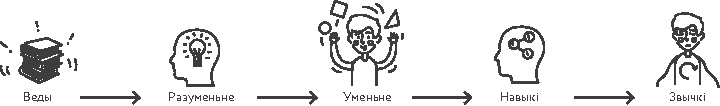
\includegraphics[scale=1.2]{willpower/ch14/2.pdf}
\end{figure*}

\textbf{Валявы рэсурс самадысцыпліны канчатковы}: стрэсы, сьпешка, недасып, недаяданьне~--- усё гэта можа аслабіць волю і зьбіць нас са шляху. Таму выпрацоўка звычак~--- гэта выкарыстаньне аўтаматычных мадэляў паводзінаў, якія вядуць нас да здароўя без штодзённых валявых выдаткаў. Зьмяніцца цяжка, бо наш мозг настроены на эканомію і аптымізацыю дзейнасьці. Чым больш звычак спрацоўвае на аўтамаце, тым меншы ціск. Калі мы любім тое, што робім, атрымліваем ад гэтага пазітыўныя эмоцыі, ідэнтыфікуем сябе са сваімі звычкамі, то робім усё лёгка, без супраціўленьняня.

\infobox{Мы самі робімся звычкай. Чым больш звычак мы ўкараняем, тым лягчэй нам гэта рабіць~--- мы папросту трэніруем ``звычку да новых звычак''.}

Пачніце з~самага малога і давядзіце гэта да аўтаматызму~--- так вы адпрацуеце навык фармаваньня звычак. Трэба толькі ``спакусіць мозг'', і ён сам зачэпіцца за задачу, а~нам застанецца адно насалоджвацца працэсам.

\textbf{Зьмена звычак}~--- справа не аднаго дня і нават месяца. Пашыраючы свой гарызонт плянаваньня, мы можам убачыць сябе ў~будучыні і прымаць тыя рашэньні, якія зробяць нас здаравейшымі і шчасьлівымі ў~доўгатэрміновай пэрспэктыве. Няўменьне так глядзець правакуе нас на імгненныя рэакцыі, якія наносяць страты здароўю. Напрыклад, заесьці стрэс, прапусьціць трэніроўку, завіснуць да глыбокай ночы на новым сэрыяле. Ці маеце вы права зрабіць гэта? Так, але тое будзе не любоў да сябе, а~патураньне, здрада вашых доўгатэрміновых мэтаў.

\subsection*{Час мяняцца}

Многім людзям страшна нешта мяняць, бо чым даўжэй існуе звычка, тым яна трывалейшая. І вось вы ў~сваёй зоне камфорту, адкуль здаецца, што ламаць сябе ня варта. Але ня верце гэтаму заспакаяльнаму голасу~--- чалавек заўсёды можа зьмяніцца да лепшага, і нават у~сталым узросьце гэтыя зьмены ідуць на карысьць.

\emph{Дасьледчыкі на працягу 18 гадоў назіралі за людзьмі, якім на той момант было ня менш за 75 гадоў. Аказалася, што адмова ад курэньня і павелічэньне фізычнай актыўнасьці нават у~такім узросьце павялічвае працягласьць жыцьця на 5 гадоў для жанчынаў і на 6 гадоў для мужчынаў.}

\begin{figure}[htb!]
  \centering
  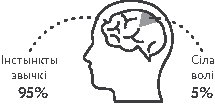
\includegraphics[scale=1.5]{willpower/ch14/1.pdf}
\end{figure}

\textbf{Мы жывыя, пакуль мяняемся, зьмены~--- гэта і ёсьць само жыцьцё.} Касьнеючы, мы становімся менш гнуткімі і адаптыўнымі, больш крохкімі~--- і нават невялікі стрэсар зможа нас зламаць. У любым узросьце будзьце дзецьмі ўнутры сябе, цікаўнымі і рызыкоўнымі!

\subsection*{Пытаньні і заданьні}

1. Якія звычкі вы хацелі б выпрацаваць? Якіх звычак вы хочаце пазбавіцца?

2. Што вы хочаце рабіць, але ня ўмееце?

3. Якое сваё азарэньне запомнілася вам мацней за ўсё?


\section{Карысьць~--- гэта задавальненьне ў~будучыні}

``Апішы мінулае, дыягнастуй сучаснасьць, прадкажы будучыню''~--- так вучыў Гіпакрат. Спробы зьмяніць сябе безь відавочнае выгады ўспрымаюцца мозгам як марнатраўства: навошта нешта мяняць, калі сёньня мне і так добра? Мы можам інвэставаць у~сябе будучыні, калі бачым гэтую самую будучыню, і яна нам падабаецца~--- ці палохае. Робячы выбар у~моманце, пытайцеся ў~сябе кожны раз, ці прынясе вам гэта карысьць у~доўгатэрміновай пэрспэктыве? Калі не, то, магчыма, яго і ня варта рабіць. Многія людзі ня хочуць нават уяўляць сябе ў~будучыні, бо гэта можа быць непрыемна для іх. Але важна рэгулярна думаць, што здарыцца з~вамі, калі вы ня зьменіцеся і будзеце працягваць кожны дзень рабіць тое, што робіце сёньня.

\emph{Ці павялічваюцца вашы рэсурсы~--- грошы, уплыў, вядомасьць, сябры, навыкі,~--- альбо вы дэвальвуецеся з~кожным годам? Ці рухаецца ваша кар'ера? Вы схуднелі ці набіраеце вагу, ці пачалі больш падцягвацца або ўжо цяжка дыхаеце, паднімаючыся па лесьвіцы? Ці пасьпяхова вы спраўляецеся са стрэсам? Ці расьце ваш «кошт»? Няма нічога страшнага ў~тым, што адказы вам не падабаюцца~--- як мінімум вы шчырыя з~сабой, а~гэта выдатны пункт адліку для зьменаў.}

У сьвеце існуе мноства заняткаў, у~якіх мы можам альбо быць пасьпяховымі, альбо застацца ні з~чым. Таму наш мозг праводзіць часта неўсьвядомлены аналіз верагоднасьці атрыманьня карысьці і на яго аснове выдае нам крэдыт матывацыі. Калі мэта прызнана годнай і шанцы на яе дасягненьне высокія, то мы напаўняемся энэргіяй і дзейнічаем. За гэты працэс адказвае дафамінавая сыстэма мозгу, а~яе нэўрамэдыятар~--- дафамін~--- можна ўмоўна разглядаць як валюту мозгу.

\textbf{Як і любую валюту, дафамін трэба зарабіць}, і яго заўсёды бракуе. У натуральных умовах дафамін выпрацоўваецца тады, калі мы робім нешта важнае і карыснае для сябе, прапампоўваючы свае навыкі і ўзмацняючы рэсурсы: прабегліся~--- дафамін, выспаліся~--- дафамін, даведаліся новае~--- дафамін і гэтак далей. З кожнае дзеі вылучаецца трохі, але якасная дывэрсіфікацыя забясьпечвае выдатнае самаадчуваньне. Зразумела, марнаваць проста так такой працай нажытую валюту мозг не зьбіраецца. І калі вы кажаце сабе «трэба»: вывучыць мову, схуднець ці пачаць бегаць,~--- мозг разумее, што гэта запатрабуе вялікіх выдаткаў энэргіі, якіх, магчыма, цяпер зусім няма і якія трэба браць у~крэдыт. Таму мозгу прасьцей сабатаваць мэты, чым вытрачацца на іх дасягненьне.

\emph{Уявіце сабе дафамінавую сыстэму як банк, а~прэфрантальную кару вашага мозгу як прадпрымальніка. Для атрыманьня крэдыту важна мець добры бізнэс-плян на будучыню: выдатную ідэю з~высокімі шанцамі на дасягненьне выніку. Чым шырэйшы ваш гарызонт плянаваньня, чым ясней вы ўяўляеце, як менавіта зьбіраецеся дасягнуць сваіх мэтаў, як будзеце спраўляцца з~узьніклямі цяжкасьцямі, тым імаверней атрымаеце крэдыт доўгатэрміновай матывацыі.}

Пакажыце «банку», што справа выйгрышная, інавацыйная і абяцае вялікі прыбытак, растлумачце, чаму менавіта вы здольныя даць гэтаму рады. Чым лепш вы ўяўляеце будучыню, тым верагодней яе дасягненьне.

\infobox{Калі вам цяжка ўявіць, што будзе з~вамі празь месяц, то ня варта і разьлічваць на матывацыю ў~доўгатэрміновых мэтах~--- мозг ня дасьць вам энэргію, калі вы жывяце адным днём. Большасьць нават ня хоча ўяўляць сябе ў~будучыні, бо гэта можа быць непрыемна. Але важна разумець, што здарыцца з~вамі, калі вы ня зьменіцеся сёньня.}

Імавернасьць невяртаньня крэдыту матывацыі настолькі высокая, што ня варта і рызыкаваць. Зьвярніце ўвагу: пад вашыя фантазіі аб тым, што «аднойчы прачнуся мільянэрам» або «выйду замуж за прынца», мозг і шэлега ламанага ня дасьць, патрэбныя толькі выразныя і рэальныя пляны.

Каб атрымаць крэдыт, трэба мець добрую крэдытную гісторыю: вы павінны мець досьвед набыцьця такіх навыкаў, няхай і ў~меншых маштабах. Змаглі бегаць і займацца раз у~тыдзень? Значыць, можна даць энэргіі і на заняткі двойчы ў~тыдзень. Крэдыт на меншую суму атрымаць нашмат рэальней, таму зьменшыце запыты і затым паступова іх падвышайце.

Для атрыманьня крэдыту патрэбны добры заклад і адсутнасьць запазычанасьцяў. Стан здароўя~--- гэта і ёсьць наш заклад. Калі мы якасна харчуемся, высыпаемся, маем разьвітую цяглічную сыстэму, кантралюем стрэс, маем доброе кола зносінаў і сацыяльны статус, то пад гэтыя рэсурсы мозг з~задавальненьнем выдасьць нам матывацыю на будучыню. Калі ўжо зь цяжкасьцю дацягваем да вечара пятніцы, ледзь спраўляемся са стрэсам, то ўся валюта мозгу будзе ісьці на забесьпячэньне штодзённага функцыянаваньня, без адкладваньня запасу на будучыню.

\subsection*{Дамаўляйцеся, а~не выбівайце сілай}

Каб атрымаць больш рэсурсаў ад свайго арганізма, мы часьцяком дзейнічаем груба, прымушаючы сябе штосьці рабіць. Але злоўжываньне словам «трэба» прыводзіць да падзеньня ўзроўню дафаміну і вялікіх валявых выдаткаў. Многія спрабуюць падмануць дафамінавую сыстэму, зьвяртаючыся да лёгкіх стымулятараў. Дафамінавая «халява»~--- гэта ўсё, што падымае ўзровень дафаміну без намаганьняў. Зьелі салодкае~--- настрой падняўся, выпілі~--- палепшылася суб'ектыўная самаацэнка. Але друк нічым не забясьпечаных грошай заўсёды прыводзіць да інфляцыі. Лішак дафамінавай стымуляцыі мозгу прыводзіць да зьяўленьня залежнасьці і яшчэ большым разладам матывацыі.

Імавернасьць атрымаць крэдыт вышэйшая, калі ў~вас ёсьць здольнасьці да таго, на што вы яго просіце. Мозг ацэньвае гэта па ўзроўні асалоды~--- усьвядомленага атрыманьня задавальненьня пры заняцьці нейкай справай. Калі вам толькі «трэба», але пры гэтым зусім не падабаецца, то, верагодна, у~крэдыце вам адмовяць. А калі вас да чагосьці моцна цягне, але вы не атрымліваеце задавальненьня, то рызыка парушэньня дафамінавай сыстэмы прыкметна ўзрастае.

Не шукайце матывацыю звонку, усё, што вам трэба, ёсьць у~вашай галаве. Сфармуйце добрую крэдытную гісторыю, патрэніраваўшыся на дробязях, навучыцеся атрымліваць задавальненьне ад мэты, устрымайцеся ад залішняй стымуляцыі, назапасьце ўнутраныя рэзэрвы. І затым стварыце рэалістычны і натхняльны бізнэс-плян па дасягненьні сваёй мэты. Тады ваш мозг дасьць вам такое натхненьне і матывацыю, што вашай энэргічнасьці можна будзе толькі пазайздросьціць. Вучыцеся не ламаць сябе, а~весьці перамовы на роўных са сваім мозгам,~--- і ўсё атрымаецца.

\subsection*{Пытаньні і заданьні}

1. Што вы думаеце пра будучыню? Ці часта вы адкладаеце нешта на заўтра?

2. Ці трымаеце балянс кароткатэрміновае-доўгатэрміновае ў~сваім жыцьці?

3. Колькі часу вы інвэстуеце ў~сябе штодзень?


\section{Тэорыя будучыні}

Мы ўвесь час хочам спазнаць будучыню~--- ад гэтага залежыць наша выжываньне,~--- таму здавён-даўна такія папулярныя варожбы, прагнозы, астролягі і да т.~п. Чым лепш мы ведаем пагрозу, тым эфэктыўней зможам да яе загадзя падрыхтавацца і больш адэкватна адрэагаваць. Таму прэфрантальныя долі заняты мадэляваньнем розных складаных сытуацый і пошукам аптымальнага рашэньня. Наш мозг будуе чаканьні і мадэлі будучыні, зыходзячы з~успамінаў аб мінулым. Аддзел мозгу гіпакамп захоўвае і ўспаміны, і праекцыі будучыні. Калі выдаліць гіпакамп, то пакутуе ня толькі памяць, але і здольнасьць плянаваць свае дзеяньні. Нядзіўна, што ўчынкі задаюць тэмп нашага жыцьця і што парадкаваньне мінулага досьведу, напрыклад, у~псыхатэрапіі, дапамагае людзям зь вялікім энтузіязмам глядзець у~будучыню.

\infobox{Чым горш вы думаеце аб сваім мінулым, тым горшай будзе і ваша будучыня. А вось маючы пазітыўныя ўспаміны, прасьцей дабівацца посьпеху.}

Па сутнасьці, чаканьні~--- гэта фантазіі нашага мозгу, яго ўяўленьні, што і як будзе адбывацца. Але гэтыя чаканьні аказваюць сур'ёзнае ўзьдзеяньне на сапраўдны момант. Нашы дзеяньні і эмоцыі знаходзяцца ў~``ценю будучыні''~--- мы можам адчуваць сябе па-рознаму ў~залежнасьці ад чаканьняў. Напрыклад, пры дэпрэсіі людзі бачаць у~будучыні толькі безвыходнасьць, нягледзячы на адсутнасьць праблемаў цяпер. І менавіта гэтая будучая безвыходнасьць прымушае іх пакутаваць ужо сёньня. Скажэньне карціны будучыні выклікае трывогу і прадчуваньні.

\textbf{Гарызонт плянаваньня ці мапа будучыні}~--- гэта чаканьні нашага мозгу, закадаваныя ў~нэўронавых контурах. Стрэс і колькасьць наяўных рэсурсаў уплывае на нашы рашэньні. Чым вышэй узровень стрэсу і ніжэй колькасьць наяўных рэсурсаў для пераадоленьня сытуацыі, тым мацней мяняецца яе ўспрыманьне.

Ва ўмовах стрэсу мозг пераходзіць на ``рэжым выжываньня'', калі гарызонт плянаваньня вельмі вузкі, і доўгатэрміновыя наступствы нашых дзеяў няважныя. Калі вы стаміліся і зьнясіленыя настолькі, што ня можаце сабрацца з~думкамі, ваш арганізм аддасьць перавагу булцы, а~не здаровай фігуры.

Гэта рэжым \textbf{``хуткага'' жыцьця}, калі выжываньне непрадказальнае, у~процівагу \textbf{``павольнаму'' жыцьцю}. У рэжыме ``хуткага'' жыцьця мы жывём адным днём, не думаючы пра будучыню. Таму разьвівайце стрэсаўстойлівасьць і вытрымку: многія людзі трапляюць у~заганнае кола стрэсу, калі яны моцна стамляюцца, і ў~іх нізкі самакантроль і няма жаданьня нешта плянаваць~--- дзень пры дні.

\emph{У рэжыме «хуткага» жыцьця мы больш спакушаемся. У банку, калі вы сядзеце запаўняць дамову на крэдыт, побач з~вамі будзе стаяць паднос з~цукеркамі, а~запаўняць паперы будзе прывабная дзяўчына~--- і не выпадкова. Чым вышэй у~вас паднімецца дафамін пры выглядзе салодкага або жаночай прывабнасьці, тым горш вы зможаце разьлічыць доўгатэрміновыя наступствы і ўмовы крэдыту.}

\begin{figure}[htb!]
  \centering
  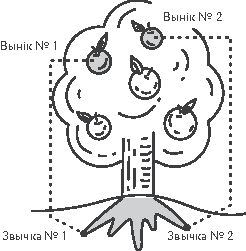
\includegraphics[scale=1.5]{willpower/ch14/3.pdf}
\end{figure}

Пры напрацаваных унутраных рэсурсах спакусы будуць на вас уплываць прыкметна слабей. Палітыкі, навіны, стрэс падаюць нам мноства сыгналаў дэфіцыту і пагрозы, што абмяжоўвае нашы паводзіны і робіць іх зьмену невыгоднай для арганізма. Усё гэта кароціць наш гарызонт плянаваньня і пераключае ў~рэжым ``хуткага'' жыцьця. Бо няма сэнсу імкнуцца худнець, калі ўсё чалавецтва можа загінуць ад каметы (вайны, крызісу, клімату, прышэльцаў, эпідэміі) у~найбліжэйшыя паўгода! Важна выконваць інфармацыйную гігіену і ўсьвядомленасьць для таго, каб захаваць матывацыю і мэтазгоднасьць зьменаў. Не паддавайцеся на правакацыі і пазьбягайце абясцэньваньня будучыні~--- гэта дапаможа вам захоўваць капітал, увагу і рэсурсы, не зьліваючы іх у~чорныя дзіркі.

Пашырайце ваш гарызонт плянаваньня: штодня надавайце час прагляду сваіх доўгатэрміновых плянаў, разважайце пра іх, пра вашу місію. Чытайце кнігі пра будучыню, прыдумляйце 5--10 крэатыўных ідэй для трэніроўкі ўяўленьня, шукайце магчымасьці і доўгатэрміновы патэнцыял у~тым, што атачае вас. Думайце пра сваю спадчыну, пра дзяцей і ўнукаў, пра экалёгію плянэты і пра ўсё, што пераўзыходзіць вас. Думайце пра карысьць здаровых звычак як пра задавальненьне~--- у~будучыні. Павярніцеся тварам да будучыні, а~не стойце да яе сьпінай, разглядаючы свой цень.

Трэніруйце футурыстычную зоркасьць. На якую колькасьць дзён наперад вы звычайна зазіраеце? Рабіце пазітыўныя прагнозы на дзень і тыдзень і ацэньвайце іх верагоднасьць. Рабіце прагнозы на розныя падзеі, напрыклад, на шпацыры падумайце, як гэтая вуліца будзе выглядаць праз 20 гадоў? Паказана, што практыка прадказаньняў сапраўды павялічвае іх дакладнасьць. Пытайце сябе, колькі разоў я падцягнуся праз месяц? Колькі грошай зараблю за месяц? Кажуць, што старасьць надыходзіць тады, калі вы кажаце больш пра мінулае, чым пра будучыню. Шукайце патэнцыял у~тым, што вакол вас,~--- гэта дапамагае ўбачыць будучыя магчымасьці і засяродзіцца на станоўчых аспэктах таго, што адбываецца, ад вонкавага сьвету да сваіх асаблівасьцяў. Трэніруйце аптымізм~--- гэта карысна для здароўя.

\subsection*{Пытаньні і заданьні}

1. Як часта вы кажаце пра будучыню? А пра мінулае? Які паміж імі балянс?

2. Як вашы чаканьні адносна будучыні ўплываюць на ваша самаадчуваньне сёньня?

3. На які тэрмін у~будучыні вы плянуеце сваё жыцьцё? Ці ёсьць у~вас гадавы, 5-гадовы, 20-гадовы пляны?


\section{Будучы Я}

Як і кім вы сябе бачыце ў~будучыні? Ці ёсьць у~вас ясны вобраз альбо толькі туманныя адчуваньні? Наколькі ясна вы можаце ўспомніць сябе ў~мінулым? Ці адчуваеце вы сувязь паміж усімі гэтымі ``я''? Навукоўцы ўсталявалі, што часта ``мы ў~сучаснасьці'' і ``мы ў~будучыні''~--- гэта амаль чужыя людзі. Мы ставімся да сябе ў~будучыні як да незнаёмца, і таму нам ня так цікава нешта рабіць для яго, напрыклад, адкладаць грошы, замест таго каб патраціць іх тут і цяпер, ня есьці сёньня салодкае, каб у~будучыні не пакутаваць ад дыябэту.

Важна разьвіваць у~сабе гэтыя навыкі~--- уяўляць сябе ў~будучыні і выбудоўваць бесьперапынную лінію свайго жыцьця, пераемнасьць паміж мінулым і будучыняй. Чым на большы тэрмін мы бачым сябе ў~будучыні і праецыруем свае задачы, тым далейшы наш гарызонт плянаваньня.

\textbf{Уменьне ўяўляць і мадэляваць} розныя сытуацыі зьвязана з~працай прэфрантальнай кары. Чым ярчэй і дакладней, эмацыйней мы бачым сябе ў~будучыні, тым мацней гэта ўплывае на нашы паводзіны сёньня. Часта ``мы ў~сучаснасьці'' і ``мы ў~будучыні''~--- гэта амаль чужыя людзі. Мы ставімся да сябе ў~будучыні як да незнаёмца, і таму мы не матываваныя нешта рабіць для яго.

Па сутнасьці, наш \textbf{самакантроль~--- гэта стрымальная праца лобных доляў}, і мы стрымліваемся ад дрэнных учынкаў, бо здольныя ўбачыць у~будучыні іх вынікі, паглядзець на сытуацыю вачыма сябе і іншых людзей, прадказаць іх рэакцыю.

Нэгатыўна ўплываюць на працу прэфрантальнай кары стрэс, стома, недасып, трывога. Усё, што кароціць сілу волі, зьмяншае значнасьць будучыні «я». Кароціць гарызонт плянаваньня і ўздым дафаміну, таму любыя моцныя спакусы і стымуляцыя зьніжаюць нашу здольнасьць рацыянальна думаць. Тыя людзі, у~каго нізкая здольнасьць убачыць сябе ў~будучыні, жывуць «тут і цяпер» увесь час, аднак у~гэтым няма ніякай рамантыкі: яны схільныя да абжорства, наркотыкаў, хамства, злачынстваў і супрацьпраўных паводзінаў. Такія імпульсіўныя паводзіны ўзьнікаюць праз няздольнасьць убачыць і ацаніць вынік сваіх дзеяньняў, людзі як быццам бы замкнёныя ў~цяперашнім дні без шанцу вырацца.

\emph{Думаць пра будучыню~--- гэта даволі энэргаёмістая задача для мозгу, таму мы яе часта пазьбягаем. Але дасьледаваньні паказваюць, што тыя людзі, якія больш і часьцей думаюць пра будучыню, эфэктыўней вырашаюць праблемы і дэманструюць больш высокі ўзровень самакантролю.}

\textbf{Ілюзія канца гісторыі.} Мы так звыклі да сваёй цяперашняй асобы, што нам здаецца~--- мы ўжо няздольныя зьмяніцца. Мы думаем, што і праз 10 гадоў будзем такімі ж, як цяпер. Але азірніцеся на мінулыя 10 гадоў: вы ж моцна зьмяніліся? Таму і ў~бліжэйшыя 10 гадоў вы зможаце дабіцца немалога прагрэсу. Пазьбягайце наіўнай ``веры ў~цуд'': праблема ня вырашыцца сама сабой. Чым мацней вы верыце ў~нешта падобнае, тым меншая імавернасьць, што вы возьмецеся за вырашэньне гэтай праблемы.

\textbf{Апішыце сябе ў~будучыні.} Для таго каб нам было прасьцей выпрацоўваць здаровыя звычкі і клапаціцца пра сябе зараз, важна ўсталяваць з~``будучым я'' сувязь, рацыянальную і эмацыйную. Для гэтага трэба максімальна канкрэтна ўяўляць менавіта сябе ў~будучыні. Звычайна, чым далей у~будучыню мы спрабуем зазірнуць, тым больш расплывістай і абстрактнай яна нам здаецца. Паглядзіце на сябе з~розных пазіцый~--- зь я-пазіцыі, збоку, зьверху і здалёку.

Апісваючы сваю будучыню, расказвайце гісторыю пра тое, як менавіта вы гэтага дасягнулі, выбудоўваючы ўвесь ланцужок дзеяў (сімуляцыя працэсу). Бо наш мозг любіць гісторыі, і для яго важна пабудаваць прычынна-выніковыя сувязі, а~ня проста дафамініць ад прыемных вобразаў. Важна быць шчырым і сумленным з~сабой. Раскажыце пра вашу працу, дом, блізкіх, паездкі, перамогі, пляны, хобі і да т.~п. Зрабіце кожную сытуацыю максімальна канкрэтнай, запазычаючы адчуваньні, пахі, смакі. Дадавайце актыўныя дзеясловы незакончанага трываньня, напрыклад ``я жыву ў~доме'' (а не ``я пабудаваў дом''), ``я працую над праектам'' (а не ``я атрымаў працу'').

Таксама апішыце дакладна час дня, людзей (у што яны апранутыя, што робяць і што гавораць) і аб'екты вакол. Хто дапамагае вам з~вашай будучыняй? Чым ярчэй і паўней апісаньне, чым больш эмоцыяў і прывязак, тым эфэктыўнейшае практыкаваньне. Задзейнічайце невэрбаліку~--- пішыце ці думайце пра гэта ў~моцнай позе, выпрастаўшыся, усьміхаючыся, ківаючы сабе для ўнутранай згоды! Важна ўсталяваць з~``будучым я'' сувязь, рацыянальную і эмацыйную. Для гэтага трэба максімальна канкрэтна ўяўляць менавіта сябе.

\textbf{Паглядзіце на сябе будучага.} Цяпер ёсьць мноства праграм, напрыклад, Faceapp, якія з~высокай ступеньню дакладнасьці могуць паказаць ваш твар у~будучыні, а~таксама змадэляваць, як паўплывае на ваш выгляд той ці іншы лад жыцьця. Калі вы бачыце сябе ў~будучыні, гэта моцна эмацыйна ўзьдзейнічае на вашу матывацыю.

Існуе даведзеная карысьць састараных фота сябе, асабліва калі вы іх раздрукуеце і будзеце трымаць пад рукой, скажам, у~нататніку.

\emph{А ў~адным з~дасьледаваньняў курцоў паказалі іх выяву праз 20 гадоў, калі яны будуць працягваць курыць. Людзі так гэтым уразіліся, што пры кантролі праз паўгода 27,5\,\% удзельнікаў, якія ўбачылі свой «твар курца», сказалі, што кінулі, але рэальна зь іх кінулі 13,8\,\% (кантроль СА), а~кінулі ў~кантрольнай групе~--- усяго 1 ,3\,\%. Гэта значыць многім кінуць дапамагло фота іх ``курца''. Сёньня вы можаце згенэраваць ваш «тлусты» і «худы», «пітушчы», «недаспаны» твар і фігуру, гэтыя фатаграфіі могуць стаць магутным каталізатарам зьменаў.}

Уяўленьне сябе ў~будучыні запускае пэўныя нэўрабіялягічныя мэханізмы, сярод якіх важным зьяўляецца актывацыя растральнай зьвіліны поясу. У адным з~дасьледаваньняў людзі, разглядаючы састараныя фатаграфіі, вырашалі больш адкладаць на сваю пэнсію. У іншым дасьледаваньні людзі, якія пісалі ліст сабе будучым праз 20 гадоў, на 74\,\% менш (у параўнаньні з~3 месяцамі) падманвалі і круцілі.

\infobox{Калі мы канкрэтна бачым будучыя вынікі сёньняшніх рашэньняў і эмацыйна рэагуем, гэта можа быць магутным матыватарам зьмяніць свой лад жыцьця.} 

\textbf{Напішыце ліст сабе будучаму.} Што вы хочаце спытаць і даведацца? Такіх лістоў можа быць шмат~--- вы можаце адправіць іх самі сабе і атрымаць праз год ці пяць гадоў па электроннай пошце. Таксама можна напісаць і ліст сабе сучаснасьці ад сябе будучыні. Або ўявіце сустрэчу з~самім сабой. Пра што вы сябе спытаеце? Пра што будзеце казаць? Гэта варта рабіць рэгулярна з~дапамогай сэрвісаў накшталт FutureMe, Letter 2 Future або выкарыстоўваючы функцыю ``адправіць пазьней'' у~Гугл і Яндэкс пошце.

\textbf{Пастаўце сябе на месца будучага ``я''.} Ацаніце свой выбар, падумайце, як бы адрэагаваў будучы ``я'' на вашы ўчынкі сёньня? Які б варыянт ён упадабаў? Як паўплываюць на вас праз 20 гадоў зьдзейсненыя сёньня ўчынкі?

\begin{figure}[htb!]
  \centering
  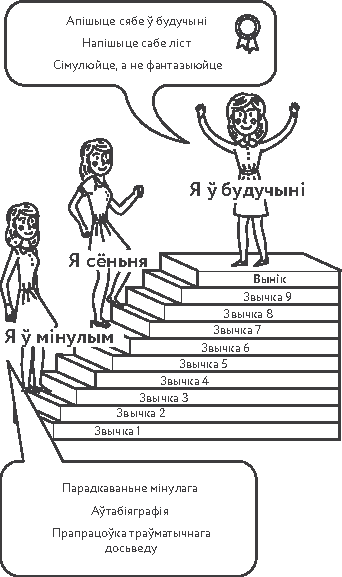
\includegraphics[scale=1.4]{willpower/ch14/4.pdf}
\end{figure}

\subsection*{Як думаць пра будучыню?}

Тыя, хто глядзеў фільм ``Сакрэт'', ведаюць адказ~--- трэба выразна ўявіць, што ты хочаш атрымаць, і прымусіць сябе паверыць, што гэта ў~цябе ўжо ёсьць. Тысячы адэптаў пазітыўнага мысьленьня і ўяўленьня па ўсім сьвеце адчайна ўяўляюць вілы, яхты і валізкі з~грашыма, але атрымліваюць толькі разлады. Чаму? Рэч у~тым, што ``фантазіі аб будучыні'' і ``сімуляцыя працэсу ў~будучыні''~--- гэта прынцыпова розныя рэчы. Фантазіруючы, мы як бы спажываем сваю будучыню, уяўляючы зьдзейсьнены факт. А завершаная задача ўжо не такая цікавая мозгу. Больш за тое, такія фантазіі~--- гэта проста дафамінавая халява, атрыманьне задавальненьня без рэальнага дзеяньня. Такія фантазіі часта зусім нерэальныя і сваю нерэальнасьць яны хаваюць пад маскай перараджэньня, тагасьветнага жыцьця або пабудовы камунізму ў~сьветлай будучыні.

\emph{Дасьледаваньні паказалі, што нерэалістычныя фантазёры маюць нашмат менш шанцаў дабіцца жаданага. Чым вышэй узровень фантазій, тым ніжэй верагоднасьць таго, што чалавек будзе прыкладаць намаганьні ў~дасягненьні мэты, і вышэй верагоднасьць няўдачы. Існуе карэляцыя паміж частатой пазітыўных фантазій і сымптомамі дэпрэсіі. Акрамя гэтага, фантазіі зьніжаюць узровень энэргіі і верагоднасьць таго, што чалавек будзе нешта рабіць.}

\textbf{Не расказвайце ўсім запар пра свае пляны}: чым больш вы дзеліцеся, тым менш верагоднасьць іх увасабленьня. Фантазіруючы і ўвесь час абмяркоўваючы свае мэты на будучыню, вы, вядома, атрымліваеце задавальненьне. Але рэч у~тым, што гэта прыводзіць да ``спажываньня будучыні'', мозг пачынае ўспрымаць гэты плян як завершаны. Многія надоўга затрымаюцца на этапе бясконцых разважаньняў, атрымліваючы задавальненьне ад працэсу. Пагаварыўшы пра дыеты і трэніроўкі, мы адчуваем палёгку, як быццам самі пазаймаліся. Нават наяўнасьць ``здаровых страваў'' у~меню можа расслабляць нас і правакаваць на паглынаньне больш калярыйных. Будзьце партызанамі~--- вядзіце таемны ЗЛЖ, бяз фота ў~інстарграме і чэкінаў у~фэйсбуку: адчуваньне таямніцы прыемнае і дапамагае прытрымлівацца звычак.

\textbf{Сымуляцыя працэсу, а~не фантазія.} Правільна не фантазіраваць, уяўляючы выніковы вынік, а~сымуляваць працэс. Сымуляцыя працэсу~--- гэта калі вы ўяўляеце, як пераадольваеце перашкоды на шляху да мэты. Напрыклад, фантазія здачы іспыту~--- гэта эйфарыя і скачкі з~залікоўкай. Сымуляцыя працэсу~--- гэта калі вы ўяўляеце сябе сфакусаванага і мэтанакіраванага, які працуе над канспэктамі, разьбірае складаныя задачы і атрымлівае задавальненьне ад прагрэсу. Уяўляць, як усе зайздросьцяць твайму прэсу,~--- гэта фантазія, а~вось плянаваць, як будзеш дабірацца да спартзалы нават у~дождж, як будзеш супрацьстаяць стрэсаваму пераяданьню,~--- гэта сымуляцыя працэсу. Такая «нэгатыўная фантазія», зьвязаная з~выяўленьнем і пераадоленьнем складанасьцяў, павялічвае веру ў~сябе, павялічвае пазітыўныя чаканьні і верагоднасьць таго, што вы даможацеся посьпеху ў~справе.

\emph{Шэраг дасьледаваньняў, дзе параўноўваліся сымуляцыі і фантазіі (у пахудзеньні, у~выпускнікоў і да т.~п.) паказалі, што сымуляцыі рэальна працуюць, а~фантазіі~--- шкодзяць.}

\infobox{Фантазія~--- гэта дафамінавая ілюзія, абязбольвальнае, для таго каб ня думаць аб рэальнасьці.}

\textbf{Мысьленны кантраст.} Зьвязвайце сучаснасьць і мінулае, калі ставіце сабе мэты: ``Я адціскаюся 20 раз, хачу адціскацца 100 разоў'',~--- кантрастуйце ``я сапраўдны vs я будучы''. Стаўце думку аб будучыні перад фактам аб сучаснасьці, ``я хачу схуднець да 60 кг, а~цяпер ува мне 120 кг''. Калі вы робіце акцэнт на тым, чаго хочаце дабіцца, а~толькі затым~--- на перашкодах, мозг факусуецца на пошуку рашэньняў дадзеных праблемаў.

\textbf{Прыдумляйце самыя розныя сцэнары.} Для мозгу карыснае павелічэньне альтэрнатыўных сцэнароў будучыні і мінулага (ах, калі б)~--- гэта важна для нашых нэўронавых сетак, канструяваньня магчымай будучыні. Вядома, ня варта ўпадаць у~скрайнасьці: думаць аб будучыні~--- гэта не трывожыцца пра яе, бо спробы паўплываць на тое, на што вы ня можаце паўплываць, толькі ўзмацняюць стрэс. Плянуйце і прадумвайце, а~потым вяртайцеся ў~сапраўдны момант зь яго задавальненьнямі. Для балянсу карысна: станоўча ставіцца і ганарыцца сваім мінулым, быць умераным у~асалодах сучаснасьцю і быць крыху арыентаваным у~будучыню.

\subsection*{Пытаньні і заданьні}

1. Які патэнцыял схаваны ў~вас і ў~тым, што вы робіце?

2. Напішыце ліст сабе будучыні.

3. Запішыце свае мэты ў~форме мысьленнага кантрасту.


\section{Упарадкаваньне мінулага}

Для кагосьці мінулае~--- гэта якар і крыніца апраўданьняў, для іншых~--- падмурак для росту, у~розных людзей розныя старты, але ўменьне мяняцца ёсьць у~кожнага чалавека. Зразумела, у~мінулым нічога нельга зьмяніць, але нашы ўспаміны аб мінулым пластычныя. Многія людзі тлумачаць свае няўдачы мінулым досьведам і ўвесь час да яго зьвяртаюцца. Наш мозг канструюе сцэнары будучыні, выкарыстоўваючы фрагменты памяці, таму важна пазітыўна і канструктыўна ставіцца да свайго мінулага і працаваць над ім, што часта і адбываецца ў~псыхатэрапіі. Перапісаўшы гісторыю нанова, прапрацаваўшы ўспаміны, якія траўмуюць, зьмяніўшы эмацыйнае стаўленьне да мінулага досьведу, зьвязаўшы разрозьненыя ўспаміны, мы пачынаем ясней бачыць сваю будучыню.

\infobox{Паміж рэальнай падзеяй і нашым успамінам можа ўвогуле ня быць нічога агульнага: успамінаючы нешта, мы кожны раз перапісваем гэта ў~памяці.}

Дасьледаваньні паказалі, што 30--50\,\% людзей лёгка ўнушыць успаміны аб падзеях, якія зь імі ніколі не адбываліся. Пры гэтым яны шчыра вераць у~іх, напаўняючы дэталямі і эмоцыямі. Навукоўцы называюць гэта «канфармізмам памяці»: калі назіраць за гіпакампам і мігдалінай з~дапамогай тамографа, можна ўбачыць, як «перазапісваюцца» ўспаміны. «Фальшывыя ўспаміны» адыгрываюць вялікую ролю ў~паказаньнях сьведак і актыўна выкарыстоўваюцца прапагандай. Напрыклад, навадныя пытаньні могуць дапамагчы сьведкам здарэньня ўпэўнена «ўспомніць» марку і колер машыны, якая зусім не прымала ўдзелу ў~ДТЗ.

Выкарыстаньне мінулага. Мы канструюем будучыню, выкарыстоўваючы фрагменты памяці. Перапісаўшы гісторыю нанова, зьвязаўшы разрозьненыя ўспаміны, мы пачынаем ясьней бачыць сваю будучыню. Я раю напісаць максімальна дэталізаваную аўтабіяграфію. Калі ў~ёй выяўляюцца сьляпыя плямы ці пэрыяды, якія вам непрыемна згадваць, можаце вярнуцца да іх пазьней. Ясная памяць аб мінулым важная для пачуцьця бесьперапыннага ўяўленьня сябе на лініі часу і, адпаведна, пазітыўнага погляду на будучыню. Чым менш у~вас яркіх успамінаў, тым складаней будаваць сімуляцыі будучыні. Многія людзі, сьвядома ці несьвядома, успамінаюць дзіцячыя гісторыі, якія іх натхняюць, свае гісторыі посьпеху. Такое мінулае~--- магутны падмурак для будучых дасягненьняў.

\emph{Аляксандру Македонскаму з~дзяцінства расказвалі гісторыю, што ён~--- сын Зеўса, і гэта, безумоўна, магутны чыньнік веры ў~сябе, які запускае эфэкт самазьдзейснага прароцтва.}

На жаль, у~многіх сем'ях выхаваньне накіраванае на прыгнечаньне дзяцей, абясцэньваньне іх намаганьняў, фармаваньне вывучанай бездапаможнасьці. Дзяцей, па сутнасьці, не выхоўваюць, а~ціснуць для атрыманьня жаданых паводзінаў. Такая памяць нэгатыўна ўплывае на ўспрыманьне будучыні.

\textbf{Шукайце апору і пазітыўныя сцэнары ў~сваім мінулым.} Вам бракуе волі да перамогі? Выпішыце ўсе ўспаміны, дзе вы перамагалі. Перажывіце іх яшчэ раз, акцэнтуючы момант на той сваёй якасьці, якую вы хочаце разьвіць у~будучыні. Прайграйце гэтыя ўспаміны, зрабіўшы іх крыху больш яркімі, пазітыўна тлумачачы няпэўнасьць. Зьбярыце набор такіх успамінаў, можна аформіць яго ў~выглядзе альбома. У маёй біяграфіі ёсьць шэраг невялікіх падзей, якія я часта згадваю, яны і сёньня зьяўляюцца для мяне крыніцай сілы: перамогі ў~алімпіядах, віктарынах, прызнаньне каштоўнасьці маёй творчасьці і да т.~п.

Успомніце рэальныя факты, пабудуйце ўспамін на аснове памяці, але пры гэтым сьмела ўключайце ўяўленьне. Тыя моманты, якія вы цьмяна памятаеце, дамалёўвайце ў~пазітыўным ключы. Такі перапрагляд успамінаў дапаможа вам зьмяніць эмацыйны зарад, знайсьці падставу сваіх дасягненьняў, апору для зьмены ў~будучыні, памяняць важнасьць падзей і зьвязаць іх прычынна-выніковымі сувязямі.

\infobox{Навукоўцы ўстанавілі, што часта нашы праблемы з~камунікацыяй і стаўленьнем да здароўя бяруць пачатак у~дзіцячым узросьце.}

У адным дасьледаваньні было паказана, што тыя людзі, хто не любіў спорт і фізкультуру ў~пачатковай школе, у~дарослым узросьце мелі сядзячы лад жыцьця і займацца фізычнай актыўнасьцю не хацелі. Гэта шмат у~чым зьвязана з~нэгатыўнымі ўспамінамі: прымус да руху, пачуцьцё няёмкасьці, насьмешкі аднакласьнікаў, траўмы, няўдалы досьвед зьніжэньня вагі і да т.~п. Для вяртаньня пазітыўнага досьведу можна ўспомніць і запісаць усе моманты з~жыцьця, дзе вам было радасна рухацца, бегаць, танчыць, усе выпадкі цяглічнай радасьці і задавальненьня ад валоданьня рухомым і гнуткім целам. Ясная памяць аб мінулым важная для бесьперапыннага ўяўленьня сябе на лініі часу. Чым менш у~вас яркіх успамінаў, тым складаней будаваць сімуляцыі будучыні.

Траўматычны досьвед важна прапрацаваць, выразна і ясна прызнаючы нэгатыўныя моманты, але й акцэнтуючы пазітыўныя. Падчас яго апісаньня карысным будзе правесьці лёгкую дысацыяцыю, замяніўшы займеньнік ``я'' на апісальны ў~трэцяй асобе, як быццам гэтую сытуацыю бачыў нехта іншы. Таксама варта выкарыстоўваць кагнітыўныя словы (думаю, лічу, таму што) і дадаць больш дэталяў. Выпісаўшы гэты досьвед на паперу, можна рытуальна запячатаць і спаліць ці закапаць. Як ні дзіўна, але ў~дасьледаваньнях паказана, што гэта дапамагае зьменшыць узьдзеяньне траўмавальных перажываньняў.

\begin{figure}[htb!]
  \centering
  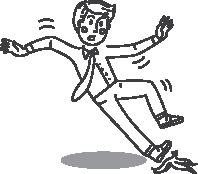
\includegraphics[scale=1.5]{willpower/ch14/5.pdf}
\end{figure}

\subsection*{Пытаньні і заданьні}

1. Напішыце сваю аўтабіяграфію.

2. Якія гераічныя гісторыі з~мінулага ў~вас ёсьць? Які траўматычны досьвед вамі не прапрацаваны? Як ён замінае вам сёньня?

3. Якія шкодныя звычкі вам не ўдаецца ўзяць пад кантроль?


\section{Этап разважаньняў і падрыхтоўкі: дайце ідэі высьпець}

Фармаваньне звычак~--- гэта пытаньне не аднаго дня, дзейнічаць трэба паступова, не кідаючыся адразу ``ў бой''. Многія людзі загараюцца ад матывавальнага артыкула, відэа ці прыкладу свайго сябра, пачынаюць капіяваць методыку і хутка выдыхаюцца. Кожны такі нэгатыўны досьвед зьменаў зьніжае вашу ўпэўненасьць у~сабе. Акрамя таго, экстрэмальныя спробы аздаравіцца нясуць сур'ёзныя рызыкі для здароўя. Зьмяніцца лёгка, галоўнае захацець па-сапраўднаму~--- такі лозунг мы можам пачуць ад розных коўчаў і матыватараў асобаснага росту. Яны ж сьцьвярджаюць, што калі ў~вас не атрымалася, то вінаватыя ў~гэтым вы і толькі вы. Насамрэч гэта ня так. Уся справа ў~кагнітыўным скажэньні~--- тыя, у~каго атрымалася, шырока разносяць інфармацыю аб сваім посьпеху, а~тыя, хто здаўся, як правіла, маўчаць.

У нас ствараецца няслушнае ўяўленьне аб пасьпяховасьці спробаў зьмяніцца~--- гэта сапраўды складана. \emph{Так, пасьпяхова ўтрымліваюць паніжаную вагу толькі 5\,\% ад тых, хто садзіцца на дыету, каля 50\,\% людзей не прымаюць прапісаныя лекі правільна, 75\,\% людзей адмаўляюцца ад сваіх плянаў. Сярод тых, хто дае сабе абяцаньні зьмяніцца ў~новым годзе, толькі 8\,\% выконваюць намеры, а~траціна здаецца ўжо ў~студзені.}

Нам важная падрыхтоўка і стараннае абдумваньне таго, што і як мы будзем рабіць, дзеля чаго мы гэта будзем рабіць і якія рэсурсы ў~нас ёсьць. Чым лепш мы прадумаем і сплянуем, тым верагодней наш шанец на посьпех~--- вылучыце адзін-два тыдні, каб сабраць больш інфармацыі і ``схадзіць на выведку'', для больш дакладнага пляна. На гэтым этапе адбываюцца неабходныя зьмены: вы падрыхтоўваеце глебу свайго розуму і кідаеце туды зерні разважаньняў і ідэй. Працягвайце паліваць іх сваёй увагай, і яны прарастуць у~выглядзе вашых дзеяньняў.

\infobox{Пастаўце сабе мэту, напрыклад, паўгадзіны ў~дзень думаць аб неабходнасьці зьмены, запісвайце асноўныя думкі ў~дзёньнік, павесьце стыкеры, якія нагадваюць пра гэта, у~лазенцы і на лядоўні.}

\textbf{Зьмены парадаксальныя}: часам патрабуюць часу, а~часам разважаньні крышталізуюцца ў~выглядзе азарэньня, якое прыводзіць да пункту невяртаньня і разуменьня, што трэба мяняцца і так далей жыць нельга.

\emph{Дасьледаваньні паказваюць, што больш за 90\,\% людзей самі, без дапамогі звонку, прымаюць рашэньне і самастойна завязваюць з~такімі шкоднымі звычкамі, як курэньне і алькаголь.} 

\begin{figure}[htb!]
  \centering
  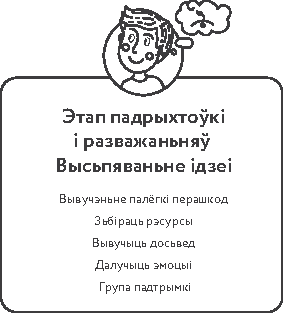
\includegraphics[scale=1.5]{willpower/ch14/6.pdf}
\end{figure}

\textbf{Што замінае зьменам?} Аналіз папярэдняга досьведу дазволіць зразумець, колькі каштуюць~--- часу, грошай, сілаў~--- вашыя трансфармацыі. Накіньце зьверху яшчэ 100\,\%, бо мы схільныя пераацэньваць свае сілы і недаацэньваць выдаткі. Ці гатовыя вы плаціць такую цану? Таксама падлічыце, чаго вам будзе каштаваць, калі вы ня зьменіце сваю звычку: колькі грошай страціце, колькі гадоў жыцьця страціце, колькі новага не даведаецеся. А такі кошт вы гатовыя заплаціць? 

\emph{Ацаніце сур'ёзнасьць свайго намеру стрэс-тэстам: хай ваш сябар паспрабуе вас адгаварыць ад зьменаў~--- ці здольныя вы супраціўляцца?} 

\textbf{Людзі зарана здаюцца.} Вельмі частая прычына няўдач~--- не даводзіць справу да канца. Рэсурсаў хапае на занадта кароткі тэрмін, хоць для фармаваньня сувязяў у~мозгу і пераходу звычкі ў~аўтаматычны рэжым патрабуецца ня меней за 66 дзён штодзённых паўтораў. Іншыя крыніцы гавораць пра 90 дзён. Калі вы выконваеце намечанае на працягу шасьці месяцаў, то верагоднасьць доўгатэрміновага посьпеху павялічваецца ў~10 разоў. Таму звычка~--- гэта маратон, а~ня спрынт, і вам трэба разьлічыць свае сілы, каб ня выдыхнуцца на паўдарогі.

\textbf{Разьлічыце свае сілы.} Уявіце сабе, што фармаваньне звычкі~--- гэта выцягваньне буйной рыбы з~вады. Тузанеце занадта моцна~--- лёска парвецца, прыслабіце~--- рыба заблытае лёску ў~хмызах. Патрэбны аптымальны ўзровень нагрузкі. Таму для зьменаў нам важна падтрымліваць усьвядомленасьць у~працэсе, і фокус на мэту. Выдаткаваўшы ў~пачатку больш увагі і сілаў на звычку, мы даможамся яе паўтарэньня ў~будучыні на аўтамаце. Трэба абраць правільны час для зьменаў, калі ў~вас ёсьць на гэта сілы і вы не адцягваецеся на іншыя энэргазатратныя рэчы. Калі ў~вас гарыць праект, то гэта не найлепшы час для старту.

\textbf{Сыстэма ці мэта.} Многія людзі ставяць сабе мэты, напрыклад, павялічыць біцэпс на пяць сантымэтраў або схуднець на пяць кілаграмаў. З пункту гледжаньня здароўя, такая пастаноўка мэт неэфэктыўная ў~доўгатэрміновым прагнозе: дасягнуўшы яе, чалавек спыняе дзеяньні і трапляе ў~вір старых звычак, якія адносяць яго назад. Завершанае дзеяньне мозг лічыць непатрэбным; калі вы схуднелі, найважнейшая частка працы яшчэ наперадзе~--- утрымаць гэтую вагу! 

\textbf{Здаровая вага і цягліцы важныя не да пачатку лета}, а~на працягу ўсяго жыцьця. Таму слушна факусавацца на тым, каб стварыць сыстэму. Сыстэму харчаваньня, якая будзе падтрымліваць здаровую структуру цела на працягу ўсяго жыцьця, стварыць крыніцу заробку на доўгатэрміновую пэрспэктыву, а~ня проста зарабіць пэўную суму.

\textbf{Прызнайце праблему цалкам, усьвядомце яе.} Калі чалавек адыходзіць ад прызнаньня, не бярэ на сябе адказнасьць, то эфэктыўнасьць прыманых мер будзе нулявая. Так, можна прымусіць кагосьці ``зьмяняцца'', але ў~гэтага чалавека зьявіцца агіда да вашых добрых намераў. Людзі спрабуюць пазьбегнуць ціску, адмаўляюць факты, выкарыстоўваюць разнастайныя ахоўныя мэханізмы псыхікі: часам аповед пра шкоду курэньня правакуе курыць больш. Многія людзі маюць фальшывую самаідэнтыфікацыю са сваімі звычкамі і ня хочуць адмаўляцца ад іх, баючыся страціць ``сябе''.

\emph{Таму так важны этап разважаньня~--- для ўсьведамленьня таго, як на нас уплываюць нашы звычкі і якія ў~нас ёсьць памылкі адносна іх і сябе.}

\textbf{Супраціў марны?} Навакольнае асяродзьдзе ўтрымлівае так шмат трыгераў, што чалавек расходуе шмат сіл на супраціў. Часта перашкаджае і таксічнае сацыяльнае асяродзьдзе, у~якім зьмены не прынятыя і не заахвочваюцца. Таму важна загадзя пралічыць, якія плюсы і мінусы вашых зьмен будуць ня толькі для вас, але і для навакольных. Зьмена асяродзьдзя ў~такім выпадку~--- важны чыньнік посьпеху. Калі асяродзьдзе вас не падтрымлівае, магчыма, давядзецца зьмяніць асяродзьдзе. Супраціў можа быць ня толькі на ўзроўні асяродзьдзя: вашы старыя звычкі будуць замінаць засваеньню новых, чым мацнейшая старая звычка, тым складаней яе «перамагчы».

\textbf{Сумневы паралізуюць.} Памятаеце прытчу пра сараканожку, якая не змагла хадзіць, калі яе папрасілі растлумачыць, як у~яе атрымліваецца адначасова перастаўляць усе сорак ног? Многія людзі пачынаюць дзейнічаць у~стане сумневаў і ваганьняў. Такая дваістасьць розуму, калі вы быццам бы хочаце зьмяніцца, а~нібы й ня хочаце~--- усё гэта чыньнікі няўдачы. На этапе плянаваньня разважайце колькі хочаце, але, калі вы пачалі працаваць па зацьверджаным пляне, ня час сумнявацца. Ваш мозг, сутыкаючыся з~нагрузкай, будзе прыдумляць сотні выкрутаў, каб не выходзіць з~зоны камфорту, і даваць вам адпор. Напэўна ў~вас ёсьць і другасныя выгады ў~вашым бягучым стане, таму магчымы самасабатаж.

\textbf{Тэорыя маленькіх перамог.} Вялікія мэты~--- гэта выдатна, яны натхняюць, і ад іх нават кружыцца галава. А вось да малых мэт многія людзі адчуваюць пагарду~--- здаецца, што гэта дробязь, няздольная нешта радыкальна зьмяніць. Ужо калі дыета, то цалкам новая ў~самай жорсткай форме~--- мы вельмі схільныя да скрайнасьцяў. Але шлях да доўгатэрміновых зьменаў ідзе менавіта праз маленькія мэты і штодзённыя перамогі.

\emph{Уявіце, што вы ідзяце пешшу да нейкага месца, разьмешчанага за дзясяткі кіламетраў. Вы ня бачыце яго, ня ўбачыце і праз гадзіну, таму неўзабаве можаце пачаць перажываць, ці ў~той бок вы ідзяце і ці варта наогул гэта рабіць~--- і сумневы загубяць вас. Але калі вы ставіце сваёй мэтай прайсьці столькі кіламетраў у~дзень, то можаце штодня сьвяткаваць перамогу, пры гэтым ведаючы, што вы становіцеся бліжэй да сваёй мэты.}

Штодзённыя перамогі заахвочваюць нас, замацоўваюць звычкі, дапамагаюць прапампоўваць сілу волі. Калі мы факусуемся на рашэньні праблемы цалкам, гэта можа выклікаць адчуваньне безнадзейнасьці, дэфіцыту рэсурсаў, зьменшыць веру ў~тое, што мы здольныя гэта зрабіць. Разьбіўшы задачу на простыя і разьвязальныя, мы пазбавімся гэтых думак. Напрыклад, многія людзі, хто адмаўляецца ад салодкага назаўжды, часьцей за ўсё зрываюцца. А вось есьці салодкае празь дзень~--- прасьцейшая ў~выкананьні задача, якая дазволіць у~два разы зьнізіць яго спажываньне, што мае станоўчы ўплыў на здароўе.

\infobox{Хочаце завязаць з~выпіўкай? Досьвед паказвае, што мэта не ўжываць алькаголь на працягу наступных 24 гадзінаў цалкам рэальная і зьдзяйсьняльная.}

Факусуйцеся на момантах посьпеху, і яны стануць каталізатарамі рэальных зьменаў. Навукоўцы высьветлілі, што самаадчуваньне прагрэсу, рухі наперад паляпшае стан чалавека, дапамагае яму заставацца больш прадуктыўным і захопленым. Толькі дзеяньне зьменіць самаацэнку і самаідэнтыфікацыю, а~ня думкі: стаўце канкрэтныя ўчынкі вышэй за разумовыя практыкаваньні і сумневы. Пачынайце тыдзень з~ударнага панядзелка, добры пачатак зарадзіць вас натхненьнем і ўпэўненасьцю на ўвесь тыдзень наперад.

\subsection*{Дысцыпліна, а~не матывацыя}

Адна з~сур'ёзных памылак у~выпрацоўцы звычак~--- гэта апірышча на матывацыю. Людзі лічаць, што трэба шукаць ці чакаць асаблівага стану гатоўнасьці рабіць тое, што трэба. Але ж наш эмацыйны фон мяняецца ў~залежнасьці ад мноства прычынаў, ад зьедзенай ежы да надвор'я за акном. Чаканьне матывацыі запускае пракрастынацыю, калі людзі кідаюць пачатае толькі таму, што адчуваюць сябе ``не прадуктыўнымі'', ``ня ў~тым настроі'', ``не ў~рэсурсе''. «Накручваць» матывацыю з~дапамогай ролікаў на ютубе, кафэіну ці разьвівальных кніг таксама дрэнная ідэя~--- гэты запал хутка выпараецца, пакідаючы вас сам-насам зь нявырашанымі праблемамі.

\textbf{Правільны падыход~--- гэта разьвіваць у~сабе дысцыпліну.} Дысцыпліна~--- гэта дзеяньні незалежна ад вашага настрою, жаданьня рабіць, пачуцьцяў, калі вы сканцэнтраваныя выключна на выніку.

\textbf{Сутнасьць дысцыпліны~--- аддзяліць выкананьне канкрэтнай справы ад вашага бягучага самаадчуваньня, рабіць нешта, нават калі вы ня можаце гэтага рабіць.}

Мозг увесь час назірае за вашымі дзеяньнямі і складае пра вас меркаваньне ў~залежнасьці ад таго, як вы паводзіцеся. Калі вы пачынаеце дзейнічаць сьмела, то паступова пачынаеце і ўспрымаць сябе адважным. Такім чынам, спачатку дзеяньне~--- толькі потым пачуцьці, а~не наадварот! Крытычна важна дзейнічаць у~рэальным сьвеце, а~не блукаць у~закутках свайго розуму, узіраючыся ў~крывыя люстэркі перажываньняў і чаканьняў. 

Факусуйцеся на мэтах, а~не на самаадчуваньні. Не на тым, як добра сябе адчуць, а~на тым, як лепш дасягнуць рэальнай мэты ў~рэальным сьвеце.

\subsection*{Пытаньні і заданьні}

1. Пачніце зьмяненьне звычкі з~этапу разважаньняў і падрыхтоўкі.

2. Якая рэальная цана зьмены? Ці гатовыя вы яе заплаціць?

3. Чаму не атрымлівалася рабіць гэта раней? Якія галоўныя перашкоды да выпрацоўкі новай звычкі вы бачыце і як іх пераадолець?


\section{Этап разважаньняў і падрыхтоўкі: зьбярыце рэсурсы для зьмены}

«Выбірай найлепшае, а~звычка зробіць яго прыемным»,~--- казаў філёзаф Плутарх. На этапе разважаньняў і падрыхтоўкі важна ня толькі вывучыць цану і пагрозы, але і сабраць рэсурсы для зьмены. Уявіце сабе шалі, на адной чары якіх усе чыньнікі, якія спрыяюць фармаваньню новай звычкі, а~на іншай~--- усё, што супраціўляецца. Чым больш у~вас будзе ў~першай чары, тым верагодней ваш посьпех. Важна загадзя падрыхтаваць усё, што вы можаце пакласьці ў~першую чару, і прыбраць ці прадумаць, як мінімізаваць узьдзеяньне зьмесьціва другой чары.

\infobox{Часам літаральна дробязь можа качнуць шалі ў~той ці іншы бок: напрыклад, у~цяжкай сытуацыі стане словаў падтрымкі ад блізкага чалавека, каб вы не здаліся і акрыялі духам.}

\textbf{Адукацыя.} Вывучыце тое, чым вы хочаце займацца. Гэта могуць быць базавыя веды, але яны важны для разуменьня спэцыфікі пастаноўкі правільных задач. Даведайцеся, якая бясьпечная хуткасьць пахуданьня, як хутка вы можаце вывучыць мову і да т.~п. Паслухайце розных экспэртаў, вывучыце разнастайныя кейсы. Апроч удалых гісторый абавязкова разгледзьце і гісторыі няўдач: знайдзіце топ-10 прычынаў, якія прыводзяць да зрываў, і да т.~п. Паглядзіце дакументальныя фільмы па тэме, прачытайце навукова-папулярныя кнігі~--- нават тое, што вам ня вельмі падабаецца, проста каб сфармаваць дакладнае ўражаньне аб прадмеце. Зьбярыце ня менш за 5--7 розных меркаваньняў~--- ад скрайнасьцяў да залатой сярэдзіны. Ня надта давярайце тым, хто будуе свае праграмы ці дае парады, засноўваючыся выключна на асабістым досьведзе,~--- такія ``гісторыі посьпеху'', як правіла, утрымоўваюць множныя кагнітыўныя ``памылкі выжылага''.

\textbf{Воля, а~не самапрымус.} Пра недахоп волі многія гавораць, а~яшчэ больш людзей блытаюць яе з~самапрымусам і спрабуюць намаганьнем прымусіць сябе нешта рабіць. Але гвалт над сабой можа разрэгуляваць працу лімбічнай сыстэмы і прывесьці да таго, што мы пачнём адчуваць агіду да таго, што робім. Разважаючы і рыхтуючыся, адчуйце сваю волю да зьменаў, жаданьне рэалізаваць свой патэнцыял. Не выпадкова я назваў кнігу ``Воля да жыцьця''~--- і мне хочацца, каб вашае жаданьне быць здаровым ператварылася ў~волю і дзеяньне!

\textbf{Што такое воля ``па-добраму''? Гэта сэнс, які рэалізуецца тут і цяпер.} Воля вынікае з~вашай натуральнай схільнасьці, цікаўнасьці, любові і самарэалізацыі, гэта як арыстоталеўская энтэлехія~--- унутраная сіла, што патэнцыйна заключае ў~сабе мэту і вынік. Або, як кажуць французы, ``пустазельле селянін выполвае фізычнымі намаганьнямі, але пшаніца ўзыходзіць толькі з~дапамогай сонца і вільгаці''. Воля зыходзіць з~унутраных запатрабаваньняў, а~ня вонкавых стымулаў. Толькі такая воля робіць вас мацнейшымі, а~не зьнясільвае.

\emph{«Воля вызваляе: такое сапраўднае вучэньне пра волю і свабоду»,~--- так сказаў Заратустра.}

\textbf{Маніторынг.} Пачніце адсочваць свой зыходны стан, нічога пакуль не прадпрымаючы. Калі ваша мэта~--- зьмяніць харчаваньне, то пачынайце весьці дзёньнік харчаваньня з~самага першага дня, калі вы хочаце пачаць трэніравацца~--- завядзіце дзёньнік штодзённай актыўнасьці. Назірайце за сабой і вучыцеся заўважаць нават невялікія зьмены~--- усьвядомленасьць вельмі важная для засваеньня звычкі. Навучыцеся адэкватна апісваць свае эмоцыі і цялесныя адчуваньні~--- гэта дапамагае быць больш сьвядомымі і паляпшае фізычнае і псыхічнае здароўе.

\emph{Калі ведзяце дзёньнік, абавязкова рабіце яго ``жывым'': падключайце зрок, слых, пах, органы пачуцьцяў. Пішыце пра мінулае, сучаснасьць і будучыню, пра іншых людзей, пра свае задавальненьні і жаданьні. Старайцеся зразумець свае ўчынкі і апісаць іх з~розных пунктаў гледжаньня.}

\textbf{Абуджэньне эмоцыяў.} Зрабіце тэму сваёй новай звычкі больш эмацыйнай, кранальнай. Крытэрый~--- гэта мурашы па скуры! Чытайце гісторыі розных людзей, вазьміце мастацкую кнігу на гэтую тэму, знайдзіце фільмы. Зьбярыце крыніцы натхненьня: фота, песьні, цытаты і да т.~п. Затым нам трэба будзе перайсьці на ўнутраную матывацыю: практыкуючы практыкаваньні з~«будучым я», які ўжо валодае патрэбнай вам звычкай, усталюйце з~сабой будучым эмацыйную сувязь, адчуйце гонар.

\emph{Для адных людзей лепш працуе пазітыўная матывацыя, а~для іншых~--- нэгатыўная, гэта шмат у~чым залежыць ад іх генэтыкі. Лепш выкарыстоўваць спалучэньне падыходаў: бізун і пернік, цягні-штурхай, морква сьпераду і морква ззаду,~--- вам напэўна знаёмыя гэтыя вобразы.}

Для пазітыўнай матывацыі выпішыце ўсе тыя перавагі, якія дасьць вам новая звычка. Для нэгатыўнай~--- усе тыя праблемы і пакуты, зь якімі вы сутыкнецеся, калі ня зьменіцеся. Нават калі гэта непрыемна, не сьпяшайцеся сканчаць~--- дайце болі затрымацца.

\infobox{Пазітыўная і нэгатыўная матывацыя для ўсіх працуе па-рознаму. Для многіх людзей толькі падзеньне на эмацыйнае дно зьяўляецца дастатковым стымулам для зьменаў.}

\textbf{Лёгкасьць і ўхіленьне перашкодаў.} Чым лягчэй вы можаце нешта зрабіць, тым імаверней вы гэта будзеце рабіць. Чым складанейшая заплянаваная справа, тым меншая імавернасьць яе ажыцьцяўленьня. Таму сфакусуйцеся на тым, як мінімізаваць марнаваньні часу, увагі, волі. Чым дакладнейшы ваш плян і менш магчымасьцяў выбару, тым лепш. Чым больш спрыяльнае асяродзьдзе для выкананьня справы, тым лепш.

Палягчайце звычку любымі спосабамі: калі ежа, то можна купіць дзённы рацыён у~службе дастаўкі. Калі фітнэс, то выбірайце трэнера і найбліжэйшую да дома залу. Калі гатаваньне, то калекцыянуйце простыя рэцэпты і напоўніце лядоўню здаровымі прадуктамі. Калі прабежка, то няхай красоўкі і форма чакаюць вас гатовымі на крэсьле ля ложка з~самае раніцы. Прадумайце загадзя ўсе магчымыя перашкоды і як вы іх будзеце пераадольваць. Напрыклад, чым вы заменіце прабежку, калі будзе дождж? Прадумайце розныя сцэнары і загадзя прапішыце алгарытм сваіх дзеяньняў. А вось у~выпадку шкодных звычак дадавайце больш перашкод. Напрыклад, схавайце абразкі сацсетак на тэлефоне ў~асобнай тэчцы са складаным паролем, прыбярыце з~дому паўфабрыкаты, для салодкіх дзён абярыце кавярню на іншым канцы горада.

\textbf{Дасьледаваньні паказалі, што, калі на кухні снэкі і прысмакі схаваць у~непранікальныя скрынкі і разьмясьціць унізе, а~карысныя прадукты~--- у~празрыстыя, на ўзроўні вачэй, то людзі аўтаматычна ядуць больш карыснага.} 

Часта прычынай няўдачы ўкараненьня прывычкі зьяўляецца адсутнасьць тэхнічных навыкаў. Калі вы ўмееце правільна прысядаць, валодаеце тэхнікай бегу, умееце гатаваць, навучаны антыстрэсавага тэхнікам, то ўжываць іх прасьцей і прыемней. Падумайце, якія навыкі вам важныя ў~авалоданьні звычкай і заплянуйце, як іх асвоіць: практычныя ўрокі кулінарыі, пастаноўка тэхнікі з~інструктарам і да т.~п.

\textbf{Выбар ключавой звычкі.} Ключавая звычка~--- гэта тая, якая, акрамя свайго прамога ўплыву, аказвае трансфармоўнае ўзьдзеяньне і на іншыя сферы вашага жыцьця, павышае ўпэўненасьць у~сабе і самаацэнку, запускае ланцуговую рэакцыю, якая цалкам мяняе лад жыцьця.

\infobox{Дзякуючы рэгулярным трэніроўкам людзі становяцца больш уважлівымі да выбару ежы, больш сацыяльна актыўнымі, менш кураць і выпіваюць,~--- і ўсё гэта адбываецца аўтаматычна, без прымусу.}

Пачаўшы падлік фінансаў, людзі аўтаматычна трацяць менш, а~працаваць пачынаюць больш прадуктыўна. Збіраючыся раз у~дзень на сямейны сьняданак, абед ці вячэру, сямейнікі паляпшаюць адносіны міжсобку, а~дзеці ў~такіх сем'ях пачынаюць лепш вучыцца і адчуваць сябе больш упэўнена. Ключавая звычка можа быць невялікай, але яна працуе як каталізатар: старанна запраўляючы пасьцелю кожнаю раніцай, мы трэніруем звычку да звычкі, павялічваем веру ў~тое, што ў~стане нешта рабіць на працягу працяглага часу. Ранішнія звычкі асабліва добрыя тым, што даюць нам зарад упэўненасьці на цэлы дзень наперад!

\textbf{Група падтрымкі.} Палегчыце сабе дзеяньне, сабраўшы групу падтрымкі~--- гэта могуць быць як дасьведчаныя сябры, да якіх вы можаце зьвярнуцца па мэнтарства, так і інтэрнэт-супольнасьць. Запрасіце іх паўдзельнічаць у~вашым маратоне па выпрацоўцы звычкі, растлумачце, якая дапамога вам патрэбная. Хтосьці можа падтрымаць вас эмацыйна, іншыя падзеляцца важнай інфармацыяй або дадуць карысную параду. 

\infobox{Абавязкова дайце справаздачу аб прагрэсе сваёй групе падтрымцы.}

Пры гэтым ня варта ўсім казаць аб сваіх пачынаньнях, бо ёсьць шмат таксічных людзей, якія будуць імкнуцца абясцэніць вашы дзеяньні. У цэлым я раю менш абмяркоўваць зь сябрамі пляны, і больш~--- канкрэтныя дзеяньні. 

\textbf{Публічнае абавязацельства, тэкставыя і фотасправаздачы ў~сацсетках}~--- гэта магутны інструмэнт матывацыі для многіх людзей. Дапаможныя ўзаемаадносіны~--- карысны рэсурс для зьмены. Тыя, хто стануць вашымі настаўнікамі і будуць слухаць і падтрымліваць вас пазітыўна, без сарказму і скепсісу.

\textbf{Вельмі важныя людзі, якія шчыра вераць у~вас, іх вера грае ролю самарэалізавальнага прадказаньня, а~вы, адчуваючы падтрымку, імкняцеся апраўдаць іх чаканьні і паказваеце рэальныя посьпехі.}

Карысныя і групы абмену досьведам, рэальныя ці віртуальныя. Часам людзі лічаць сваю праблему ўнікальнай, зьвязанай з~асаблівасьцю асобы: ``У мяне не атрымалася, таму што я такі'',~--- але вывучэньне досьведу іншых людзей паказвае, што многія сутыкаюцца з~такой жа праблемай, яна не зьяўляецца асабіста вашай. Гэта дапамагае ўспрымаць яе як тэхнічную і стымулюе шукаць алгарытм для яе рашэньня, выкарыстоўваючы досьвед асяродзьдзя.

\subsection*{Пытаньні і заданьні}

1. Якія рэсурсы ў~вас ёсьць для выпрацоўкі звычкі?

2. Ці ёсьць у~вас эмацыйны зарад на новую звычку? Ці натхняе яна вас?

3. Якая звычка для вас зьяўляецца ключавой?


\section{Спакушэньне мозгу}

Напэўна, многія людзі сутыкаліся з~тым, што яны быццам бы хочуць зьмяніцца або пачаць нешта рабіць, але «галавой», а~не «сэрцам». Нічога не адбываецца менавіта таму, што кагнітыўнае жаданьне, разуменьне праблемы не прыводзіць да дзеяньня. Энэргія для дзеяньня нараджаецца ў~падкоркавых дафамінавых цэнтрах. Калі мы сапраўды хочам нешта зрабіць, наша ўвага сфакусаваная на прадмеце жарсьці, мы думаем і рухаемся толькі да яго, нішто ня можа нас адцягнуць або спыніць. Таму хачу расказаць аб выпрацоўцы звычак ``зь любові''. Для таго каб не паглыбляцца ў~нэўрабіялягічныя нэтры, я спрошчана разьбяру ўзаемадзеяньне прэфрантальнай кары мозгу (аналіз, воля, самапрымус, самакрытыка, тармажэньне) і дафамінавую сыстэму (цяга, прыхільнасьць, агіда і да т.~п.).

\textbf{Прынцып «зь любові».} Для доўгатэрміновага посьпеху важна любіць тое, што ты робіш. Гучыць гэта проста, але, як мы ўсе ведаем, любоў~--- штука складаная, а~пасьля прымусу застаецца толькі агіда: бацькі, што запіхваюць брокалі ў~дзяцей, якія плачуць, не даб'юцца ад іх любові да здаровага харчаваньня.

\emph{«Сілаю ня быць мілаю», кажа народная мудрасьць, а~Марк Твэн скептычна заўважаў, што «адзіны спосаб захаваць здароўе~--- есьці тое, чаго ня любіш, піць тое, што не падабаецца, і рабіць тое, чаго ня хочацца рабіць.}

\textbf{Няўжо мы вымушаныя так сябе прымушаць? Вядома не, можна і трэба ўкараняць новыя звычкі палюбоўна.Спакусіце мозг за тры этапы: прыцягненьне, камфорт, самаідэнтыфікацыя. Такім чынам, паехалі.}

\subsection*{Прыцягненьне}

\textbf{На гэтым этапе знайдзіце тое, што прыцягвае ўвагу}, дражніць, чапляе. Звычайна гэта чыньнікі, зьвязаныя са значнасьцю: падумайце, як новая звычка зробіць вас багацей, прыгажэй, энэргічней і павысіць ваш статус у~вачах іншых людзей, чаму гэта так крута і важна. Напрыклад, магчымасьць бліснуць красамоўем перад іншымі можа быць выдатнай зачэпкай для пачатку вывучэньня мовы. Ператварайце практыку ва ўзнагароду: прыгожа апранайцеся, калі практыкуеце звычку, вывучыце любімую песню на замежнай мове ці сыграйце хіт свайго юнацтва, калі вучыцеся граць на інструменце. На трэніроўцы слухайце любімы падкаст і апранайце прыгожую форму, робячы адначасова з~заняткамі некалькі прыемных рэчаў, вы палюбіце і трэніравацца.

Паспрабуйце пагуляць са сваёй задачай, вывучыце яе з~розных бакоў у~пошуку цікаўнага і пацешнага. Пагартайце кнігу, панюхайце яе, знайдзіце цікавыя карцінкі ці фразы ў~любым месцы, дайце зачапіць сябе. Пачынайце зь лёгкасьці і спантаннасьці~--- так вы можаце неўзаметку ўцягнуцца і далей займацца без прымусу. Як новая звычка палепшыць вас і чаму гэта так важна? Уявіце, як вымаўляеце яркую прамову перад іншымі. Гэта можа быць выдатнай зачэпкай для пачатку вывучэньня мовы.

\subsection*{Камфорт}

\textbf{Другі этап~--- гэта стварэньне эмацыйнага камфорту.} Тут важная эмацыйная бясьпека: дзейнічайце натуральна і кангруэнтна, упэўнена асвойвайце звычку ў~камфортных умовах, дзе вам можна спрабаваць, памыляцца, выпраўляцца. Часта людзям цяжка ўтрымліваць здаровыя звычкі, калі яны сутыкаюцца з~кпінамі навакольных, няхай гэта будзе заняткі спортам ці пахуданьне. Група падтрымкі, камфортнае асяродзьдзе важныя, каб мы маглі сфакусавацца на звычцы, а~не турбаваліся аб тым, што пра нас падумаюць навакольныя.

\begin{figure}[htb!]
  \centering
  
\includegraphics[scale=1.5]{willpower/ch14/7.pdf}
\end{figure}

\subsection*{Самаідэнтыфікацыя}

На трэцім этапе, калі ўзьнікае дафамінавая цяга, звычка пачынае вас прыцягваць, вы думаеце і прадчуваеце яе,~--- тут адбываецца \textbf{самаідэнтыфікацыя} зь ёй, зьліцьцё~--- вы ўжо бачыце сябе як чалавека, які валодае ёй. Самаідэнтыфікацыя са звычкай дазваляе вам залучыць яе ў~свае асабістыя межы, вы ўспрымаеце яе як свой уласны стандарт. Цяпер вы ня проста чалавек, які прымушае сябе схуднець,~--- вы выконваеце свае асабістыя высокія стандарты здаровага харчаваньня, вы ня проста прымушаеце сябе хадзіць у~залу~--- вы ўжо жывяце спортам, не ўяўляеце сябе бяз гэтага.

\textbf{Як і ў~любых адносінах}, заахвочвайце ў~сабе добрае да сябе стаўленьне, а~дрэннае~--- спыняйце. Спакушэньне мозгу~--- гэта заўсёды эмацыйная, а~не рацыянальная праца. Можна доўга пераконваць сябе лягічнымі аргументамі, як у~выпадку шлюбу па разьліку, але гэта не прывядзе да каханьня. Прымушаючы сябе, мы можам справакаваць сытуацыю, калі заняткі спортам забіраюць больш сіл, чым даюць, прымус сябе да здаровага харчаваньня забірае больш сіл, чым дае~--- але такое становішча спраў няправільна. Таму спакушайце мозг, ствараючы прыемную атмасферу~--- усё роўна, што будзе пэўнай прычынай гэтых эмоцыяў, мозг заўсёды прыдумае, як іх рацыяналізаваць.

\emph{Дасьледаваньні паказалі, што людзі не зусім ясна могуць зразумець прычыны сваіх эмацыйных станаў, але лёгка іх для сябе тлумачаць. Гэта значыць, што, калі вам прыемна вучыць ангельскую мову з~любой прычыны: падабаецца ваш сусед па парце, від з~акна або любая іншая ірацыянальная рэч,~--- то вы будзеце рабіць гэта з~задавальненьнем.}

Для таго каб захоўваць \textbf{эмацыйны камфорт}, важна пазьбягаць нуды ці занадта моцнай стомленасьці. Як назойлівасьць у~заляцаньні можа лёгка спудзіць аб'ект вашай увагі, так і ў~новым распачынаньні не захапляйцеся адразу занадта моцна. Займайцеся да таго моманту, пакуль ёсьць цікавасьць. Як толькі яна згасла ці пачала зьніжацца, спыняйце: важна скончыць на ўздыме! Варта нават штучна абмяжоўваць час трэніроўкі, заканчваць на яркай эмоцыі і зь невялікім шкадаваньнем: маўляў, эх, недатрэніў! Няхай ваша практыка будзе як флірт~--- лёгкая, рамантычная, выпадковая і з~вар'яцінкай. Не зазірайце ў~будучыню, бегайце ці займайцеся сёньня, а~не пажыцьцёва. Практыкуйце разнастайнасьць, розныя сцэнары, рознае адзеньне. Прыдумайце маршрут бегу для кожнага дня, майку для нядзелі, дайце імёны сваім гірам, красоўкам, ноўтбуку або ручцы. Творчасьць і крэатыўнасьць заўсёды прыцягваюць увагу: нам патрэбная цікавасьць, а~ня лёгіка!

\emph{Нудна гуляць? Прайдзіце ці прабяжыце гэтыя сто мэтраў як Чабурашка, як Чаплін, як чабурэк~--- дайце волю ўяўленьню, каб выпрабаваць эмоцыі.}

Вельмі часта наша ``ня хочацца''~--- гэта не сапраўднае нежаданьне, а~фрустрацыя, калі мы ў~выніку няўдалага досьведу або ў~страху пацярпець няўдачу забараняем сабе адчуваць задавальненьне ад чаго-небудзь, падманваем сябе і распавядаем сабе байку пра ``зялёны вінаград''. Таму не паддавайцеся на ілюзорную самадастатковасьць: насамрэч усім людзям ідзе на карысьць добрая фігура, здаровы сон, прыемная кампанія, высокі даход.

\textbf{Оптымум матывацыі, або Не перадушыце цікавасьць.} Залішняя зацыкленасьць і залішне высокі ўзровень узрушанасьці могуць пагаршаць нашу прадуктыўнасьць і замінаць засваеньню звычкі.

\emph{Навукоўцы Робэрт Еркс і Джон Додсан ў~1908 годзе ўсталявалі: для таго каб навучыць жывёл праходзіць лябірынт, найбольш спрыяльнай зьяўляецца сярэдняя інтэнсіўнасьць матывацыі. Дасьледаваньні людзей паказалі такую ж заканамернасьць: слабая матывацыя недастатковая для посьпеху, але і залішняя шкодная, паколькі спараджае непатрэбнае ўзбуджэньне і стрэс. Закон Еркса--Додсана абвяшчае, што існуе оптымум матывацыі, які можна ўсталяваць экспэрымэнтальна. Для задач рознай цяжкасьці максімальная рэзультатыўнасьць дасягаецца: для складаных задач пры слабой матывацыі (2--3 балы па 10-бальнай шкале), для сярэдніх~--- пры сярэдняй (каля 5) і простых~--- пры высокай (7--8 і нават вышэй).}

\infobox{Гаворачы аб здароўі, важна казаць аб сіле і жарсьці, а~вось усякая іпахондрыя зусім не сэксуальная.}

Карысна зьменшыць важнасьць таго, чым вы займаецеся: пасьмяяцца зь сябе, выпусьціць пару, зьменшыць ціск. Я як лекар люблю мэдыцынскі гумар, хаця ён можа здацца грубым, але гэта эфэктыўны спосаб пазьбегнуць выгараньня.

\textbf{Дафамінавае прэкандыцыянаваньне.} Як ужо гаварылася вышэй, за нашу ўвагу канкуруе мноства стымулаў. Самы просты спосаб сфакусаваць увагу на звычцы~--- гэта абмежаваць канкуруючыя стымулы. Калі хочаце есьці па-сапраўднаму, то і качан капусты здасца вам асалодай у~адсутнасьці іншых крыніц ежы. Калі вы практыкуеце ўмеранасьць, пазьбягаеце залішняй дафамінавая стымуляцыі, звычайныя рэчы будуць для вас прывабнейшыя.

\emph{Гэта рэцэпт аднаго вядомага пісьменьніка~--- калі ён не хацеў пісаць, то замыкаўся ў~пакоі, дзе нічога няма, акрамя паперы і асадкі. Нуда рабіла сваю справу~--- рана ці позна цікавасьць вярталася.}

Пра шчасьлівае каханьне вершаў ня пішуць, бо ўсе сілы сыходзяць на само каханьне. Устрыманьне дапаможа вам сублімаваць увагу і энэргію, распаліць агонь матывацыі. Стварыце сабе ``голад'', абмяжуйце час на звычку, тады яна стане задавальненьнем сама па сабе.

\textbf{Біяхакінг самаідэнтыфікацыі.} Дасьведчаныя спакусьнікі ведаюць, што ваш бягучы эмацыйны стан праецыруецца на тое, што вы робіце. Калі вы ў~добрым настроі, то музыка і ежа, якую вы слухаеце і ясьце, пададуцца вам прыемнымі і смачнымі. Мозг прымае рашэньні і робіць высновы, назіраючы за вашай фізыялёгіяй. Калі мы займаемся нечым і нам добра, то мозг лічыць, што ў~нас да гэтага ёсьць здольнасьць.

\textbf{Таму, калі вы створыце аптымальныя ўмовы для выпрацоўкі звычкі, вам будзе нашмат прыемней ёй займацца.}

Зьмяняючы дзеяньне, зьмяняем самаідэнтыфікацыю: калі нам даецца нешта лёгка, значыць, мы таленавітыя ў~гэтым; калі мы робім нешта без прымусу, дык гэта важна для нас; калі нам лёгка на чымсьці сфакусавацца, мозг лічыць, што гэтая тэма нам цікавая. Прыемныя адчуваньні становяцца базай для здольнасьцяў. Гэта датычыцца і самаідэнтыфікацыі: мы лічым сябе тым, што мы робім з~задавальненьнем.

\emph{Хочаце адчуць уцягнутасьць у~нейкую тэму? Выступіце з~публічнай прамовай наконт гэтага, і вы адчуеце, як зьмянілася ваша стаўленьне.}

Тыповай ілюстрацыяй зьяўляецца прыклад прэзідэнта Бэнджаміна Франкліна, які ператварыў свайго ворага ў~сябра, папрасіўшы ў~таго пачытаць рэдкую кнігу. Той пагадзіўся~--- і парадаксальным чынам яго варожасьць зьнікла. Чаму? Мозг мяняе ацэнкі, грунтуючыся на дзеяньнях. Звычайна мы даём кнігі сябрам, раз ты даў яму кнігу, значыць ён~--- сябар.

\subsection*{Пытаньні і заданьні}

1. Што больш за ўсё чапляе вас у~тым, што вы хочаце асвоіць?

2. Нічога не рабіце і не прымушайце сябе. Нагуляйце апэтыт і цікавасьць да звычкі.

3. Прымерце звычку як частку сваёй асобы. Ці падабаецеся вы сабе, калі гэта робіце? Прымерце шкодныя звычкі да сябе, ці падабаецеся вы сабе, калі іх робіце?


\section{Этап плянаваньня}

Такім чынам, пасьля таго як вы высьпелі, старанна абдумалі звычку, сабралі неабходныя для яе рэалізацыі інфармацыйныя, эмацыйныя, матывацыйны, сацыяльныя рэсурсы, прыходзіць час скласьці канкрэтны плян і перайсьці да дзеяньняў. Наперад, прэч з~пасткі пэрфэкцыянізму і хранічных разважаньняў!

Адзін з~сакрэтаў таго, чаму людзі з~больш высокім статусам часьцей спрабуюць нешта зрабіць,~--- гэта большая колькасьць рэсурсаў у~іх. Можна шмат разоў спрабаваць, бо нават у~выпадку няўдачы застаюцца і іншыя магчымасьці. Чым больш рэсурсаў, тым на буйнейшую мэту можна замахнуцца.

Цяпер, калі вы прааналізавалі і сабралі ўсе свае рэсурсы, вы можаце адчуць упэўненасьць. У вас ёсьць рэсурсы для зьмены, зараз вам трэба скласьці добры плян дасягненьня мэты. Плянаваньне дапаможа вам дакладна прытрымлівацца вызначанага маршруту, трымаць навідавоку ўсе магчымасьці, пры павелічэньні стрэсу мець адыходныя шляхі на загадзя прадуманыя «ўмацаваньні», і пазьбягаць самасабатажу.

\subsection*{Фізыялягічна адэкватная мэта}

Ёсьць стандартныя крытэры правільнай мэты~--- гэта мадэль \textbf{SMART-мэты}. 

\textbf{Specific} (канкрэтная): якімі вы будзеце праз 90 дзён, характарыстыкі вашых паводзінаў, а~не адчуваньняў. 

\textbf{Measurable} (вымерная): адназначныя канкрэтныя вызначэньні на фактах, а~не ацэнках. Напрыклад, сантымэтры ці вага, сілавыя паказьнікі ці глыбіня сну. 

\textbf{Achievable} (дасягальная): хуткасьць дасягненьня здаровых звычак залежыць ад вашага зыходнага стану, крыху ніжэй разьбяром гэта падрабязьней. 

\textbf{Relevant} (значная): адпаведнасьць мэты вашай маралі і каштоўнасьцям. 

\textbf{Time bound} (абмежаваная ў~часе): займацца сваёй мэтай не менш за 90 дзён, у~ідэале~--- кожны дзень, фармуючы непарыўны штодзённы ланцуг дзеяньняў. 

\emph{Ваш плян павінен быць сфармаваны максімальна канкрэтна. Што я буду рабіць? Падцягвацца на турніку ў~калідоры. Як? Да адмовы. Калі? Кожны раз, калі я зьбіраюся зайсьці на кухню.}

Такім чынам, вы запісалі сваю мэту і вам падабаецца, як яна гучыць. Напрыклад, схуднець на 30 кг за месяц да лета. Але што тут ня так? У фізыялягічных працэсаў ёсьць свае хуткасьці зьмены, зададзеныя як індывідуальнай генэтыкай, так і зыходным станам. Існуе свая хуткасьць росту цягліцаў~--- яна адрозьніваецца ў~мужчынаў і ў~жанчынаў і залежыць ад узроўню тэстастэрону, тэхнікі, харчаваньня, сну і іншых чыньнікаў. Бясьпечная хуткасьць пахуданьня вар'іруецца ў~дыяпазоне 0,5--1 кг у~тыдзень, не хутчэй. Больш высокія хуткасьці небясьпечныя сур'ёзнымі пабочнымі эфэктамі для здароўя, рызыкай хуткага набору вагі (эфэкт рыкашэту, эфэкт ё-ё) пры спыненьні дыеты, гарманальнымі парушэньнямі (парушэньне мэнструальнага цыклу і да т.~п.), дэпрэсіямі, астэапарозам. 

\emph{Чым вышэй ваша зыходная вага, тым хутчэй вы станеце худнець, а~вось апошнія 5 кг будуць сыходзіць павольней. Калі ў~вас ужо разьвітая цяглічная маса, то прагрэсаваць вы будзеце павольней, чым навічок, толькі што прыйшоў у~залу.}

Прырост фізычнай нагрузкі трэба рабіць ня больш, чым на 5--10\,\% у~тыдзень, каб пазьбегнуць залішняй нагрузкі і адсочваць сваю хуткасьць аднаўленьня. На стабілізацыю псыхічнага стану і выхаду з~дэпрэсіі таксама патрабуецца час, бо працэс нэўраплястычнасьці не так хуткі. Нават калі вы зьмянілі свой лад жыцьця, не чакайце імгненных вынікаў. Бо для таго, каб аднавіць адчувальнасьць тканін да інсуліну, да лептыну, аднавіць адчувальнасьць дафамінавых рэцэптараў, якія вы спалілі «лёгкім» дафамінам,~--- на ўсё гэта патрабуюцца месяцы.

\subsection*{Ацаніце свае сілы}

Мы, людзі, часта пераацэньваем і зыходны стан свайго здароўя, і свае сілы: нам здаецца, што зьмяніць сваю штодзённую руціну вельмі лёгка, але гэта ня так. 

\emph{Дасьледаваньні паказваюць, што людзі на 40--80\,\% пераацэньваюць узровень сваёй фізычнай актыўнасьці, да 30--40\,\% прыніжаюць спажываны каляраж, ня могуць правільна падлічыць колькасьць прыёмаў ежы ў~дзень, недаацэньваюць праведзены ў~смартфоне час, якасьць адносін зь іншымі, неадэкватна ацэньваюць свае фінансавыя вытраты і працоўныя навыкі.}

Для цікавасьці, спытайце ў~тых, хто добра вас ведае, пацягнеце вы такое зьмяненьне ці не, і сумуйце іх адказы. Варта адзначыць, што звычайна мы займаемся слабей, калі няма выразнага вонкавага кантролю. Прысутнасьць трэнера прымушае нас мацней выкладвацца. Аб'ектывізуйце вашыя звычкі ў~лічбах, бо калі няма іх росту, то няма і прагрэсу. 

\textbf{Для таго каб ацаніць рэалістычнасьць, вы можаце спытаць у~розных спэцыялістаў, наколькі верагодна ў~вашым выпадку дасягнуць нейкай мэты за нейкі час. Супаставіўшы розныя адказы, вы атрымаеце шчырую карціну.}

\textbf{Запішыце плян.} Не трымайце ўсё ў~галаве, завядзіце тэчку для кожнай звычкі. Вы заўсёды можаце зьвярнуцца да яе, каб асьвяжыць матывацыю. Захоўвайце ў~пісьмовым выглядзе мэту і падмэты, плюсы і мінусы зьмены, станоўчую і адмоўную матывацыю, трыгеры, сьпіс удзельнікаў вашай групы падтрымкі, магчымыя сцэнары і плян па пераадоленьні магчымых няўдач. Няхай тут жа будзе ўсё, што вас матывуе: выявы, тэкст абавязацельства перад сабой, ілюстрацыі, цытаты і любыя іншыя крыніцы натхненьня. Вы павінны, як дасьведчаны казанова, «закружыць галаву» свайму мозгу новай звычкай, каб ён у~яе закахаўся і ня змог пярэчыць зьменам.

\textbf{Нягледзячы на ўсеагульны скепсіс наконт навагодніх абяцаньняў, асаблівы пачатак важны для звычкі. Няхай гэта будзе асаблівы дзень і асаблівы першы тыдзень пачатку новай звычкі.}

\subsection*{Пытаньні і заданьні}

1. Ці ёсьць у~вас канкрэтная мэта для фармаваньня звычкі?

2. Ці фізыялягічная мэта? Ці стане ў~вас на яе рэсурсаў?

3. Ці ёсьць у~вас плян у~пісьмовым дэталізаваным выглядзе?


\section{Прынцып маленькіх мэтаў}

Штодзённыя перамогі вельмі важныя для пасьпяховага старту, калі вы выпрацоўваеце звычку. Але што рабіць, калі фінальная мэта далёка, а~перамогі і натхненьне патрэбныя ўжо сёньня? Як гаварылася вышэй, для гэтага трэба глябальную мэту разьбіць на падмэты.

\infobox{Маленькія мэты~--- гэта выкананьне пунктаў па чарзе, у~адпаведнасьці з~плянам, прычым ня ў~поўным аб'ёме, стрымліваючы свой энтузіязм. Многіх людзей маленькія мэты ня моцна натхняюць, таму адначасова трымайце ў~розуме сваю глябальную мэту і разглядайце маленькія мэты як крокі да вялікай.}

Выбірайце тыя маленькія мэты, якія простыя ў~выкананьні і даюць найбольшую аддачу, напрыклад, пачынайце харчаваньне не з~радыкальнай зьмены дыеты, а~з рэгулярнага здаровага сьняданку. Гэта проста заплянаваць, проста ажыцьцявіць~--- але эфэкт вялікі.

\emph{Яшчэ раз падкрэслю, што менавіта ``ранішнія'' звычкі зараджаюць энэргіяй і матывацыяй на цэлы дзень наперад.}

Сапраўдная маленькая мэта здаецца настолькі лёгкай, што яе прасьцей зрабіць, чым не зрабіць. Я часам чую ад кліентаў, што ў~іх няма часу на практыкаваньні, і пытаю, ці ёсьць у~іх 5 хвілінаў раніцай. Яшчэ ніхто не адказаў, што не можа вылучыць сабе 5 хвілінаў. Маленькія мэты ператвараюцца ў~маленькія звычкі. Як кропля точыць камень, яны павольна, але дакладна разгортваюць ваш лад жыцьця ў~правільным кірунку.

Пасьлядоўнасьць мэтаў трэба выбіраць, зыходзячы з~плянаванай глябальнай мэты. Калі ваша мэта~--- сілавыя віды спорту, то спачатку важна асвойваць тэхніку з~пустым грыфам і ўмацоўваць мышцы кара. Калі гэта харчаваньне, то можна навучыцца гатаваць некалькі базавых страваў. Сабраліся бегчы маратон? Пачніце з~вызначэньня пульсавых зон. Ацаніце, якіх вам навыкаў бракуе. Гэта вельмі важна, каб не было расчараваньня на стадыі актыўнага дзеяньня. І так, на гэтым этапе вы можаце экспэрымэнтаваць: зрабіць ``азнаямленчыя'' спробы, наведаўшы адкрытыя заняткі моўнай школы або паспрабаваўшы розныя віды трэніровак. Існуюць дзясяткі розных відаў заняткаў, трэніровак, школ, сыстэмаў мэдытацыі і стрэсаўстойлівасьці, клюбаў бегу, спартыўных сэкцыяў~--- паспрабуйце розныя, абярыце тое, што падабаецца, і тое, што зручна.

\subsection*{Не спусташайцеся на першым этапе}

Пасьля таго, як разьбілі вялікую мэту на дробныя, зьменшыце нагрузку яшчэ мацней. У самым пачатку наша задача трэніраваць звычку да звычкі, штодня выконваючы намечанае. І сачыць за тым, каб ня вычарпацца, інакш мы страцім смак да мэты. Маленькія мэты ня толькі забясьпечваюць нам паток штодзённых перамог, але і дапамагаюць структураваць час, даюць пачуцьцё руху наперад. Плянуйце звычку на абмежаваны час~--- няхай гэта будзе тыдзень здаровага харчаваньня або 20 дзён трэніровак. А затым вы самі вырашыце, варта яе працягваць ці не.

У штодзённай практыцы важна не губляць з-пад увагі канчатковую мэту, але факусавацца трэба менавіта на наступным кроку. Альпініст думае, куды паставіць нагу зараз, а~не як ён будзе радавацца на вяршыні.

\emph{Калі ісьці да гары, разьмешчанай удалечыні, то нават праз гадзіну хады яна ня здасца бліжэй. Але калі лічыць крокі, дык мы ведаем, што на некалькі тысячаў крокаў яна наблізілася.}

\textbf{Мінімальнае выкананьне заданьня.} Які самы мінімальны посьпех прынясе карысьць для канчатковага выніку? Чакайце ад сябе самага малога: пастаўце мінімальны плян прачытаць 1 старонку, а~далей~--- толькі па жаданьні. Няма жаданьня падцягвацца 15 разоў? Пастаўце мінімум у~адно падцягваньне. Няма жаданьня бегчы па стадыёне? Пастаўце мінімальны плян пешшу прайсьці адно кола. Важна шукаць і ўжываць усё, што можа прынесьці задавальненьне ад гэтай звычкі: як толькі вы пачняце цешыцца звычцы~--- лічыце, вялікая частка працы зробленая.

\emph{Канцэпцыя мінімальнага заданьня дапаможа вам пераадолець параліч волі і пачаць дзеяць.}

\textbf{Правіла маленькіх мэтаў} мае на ўвазе, што яны не проста маленькія, але і простыя. Спрашчаць мэту мы можам рознымі спосабамі, зьніжаючы нагрузку, вытрату часу, сіл, грошай, увагі і да т.~п. Напрыклад, 20 хвілін практыкаваньняў дома, а~не доўгая дарога ў~залу. Палягчэньне рутыны: ад гатовага рацыёну да сабранай у~залу торбы спрашчае задачу, зьмяншайце «трэньне» і хай усё ідзе як па масьле. Іншы спосаб~--- падвышаць здольнасьць рабіць нешта. Калі задача даведзена да аўтаматызму, то мы лёгка робім яе нават стомленыя і галодныя. Спрасьціць мэты мы можам, калі ўпляцём іх у~свой рэжым дня: зручна, калі вы групуеце карысныя звычкі, выконваючы іх пасьлядоўна ва ўсталяваны час. Так лёгка можна згрупаваць свае ранішнія і вечаровыя звычкі ў~ланцуг пасьлядоўных дзеяньняў: зарадка~--- душ~--- мэдытацыя~--- сьняданак і да т.~п.

\textbf{Аптымальны час і месца.} Узровень нашай энэргіі вагаецца ў~залежнасьці ад часу дня, узроўня стрэсу, месцы, асяродзьдзя і да т.~п. Як хвалі, так і наша энэргія вагаецца, а~значыць і мяняецца верагоднасьць дзеяньня. Важна выбіраць аптымальны момант для засваеньня звычкі, як правіла, гэта першая палова дня, невялікі ўзровень стрэсу, добры сон. Але для розных людзей гэта можа быць розны час~--- важна назіраць за сабой і лавіць пэрыяды, калі ў~вас нараджаецца жаданьне прытрымлівацца звычкі, якую вы выпрацоўваеце.

Падсумоўваючы невялікія звычкі, мы павялічваем хуткасьць і маштаб зьменаў. Гвалтуючы і прымушаючы сябе, мы будзем сабатаваць свае ж дзеяньні, крытыкаваць, ненавідзець сябе і кідаць пачатае, тым самым толькі разьвіваючы вывучаную бездапаможнасьць. Кожная маленькая звычка можа стаць вашым трамплінам, каталізатарам зьменаў. Паверыўшы ў~сябе, у~сваю здольнасьць мяняцца, вы з~большай упэўненасьцю возьмецеся і за больш амбітныя мэты, бо цяпер у~вас ёсьць гісторыя посьпеху.

\subsection*{Пытаньні і заданьні}

1. Разьбіце мэту на маленькія і простыя крокі і запішыце іх.

2. Якое мінімальнае дзеяньне трэба выканаць для падтрыманьня звычкі?

3. Якое ідэальнае месца і час для вашай звычкі?


\section{Парадокс забаронаў}

«Хто магутны? Той, хто можа перамагаць свае благія звычкі»,~--- сьцьвярджаў Бэнджамін Франклін. Пазбавіцца ад шкодных звычак бывае нават больш карысна, чым набыць здаровыя. Звычкі так глыбока пускаюць карані ў~нашай псыхіцы, што выкараніць іх вельмі складана. Каб пазбавіцца ад іх, людзі часта ўступаюць на шлях забарон і абмежавальных паводзінаў. На жаль, часта гэта можа даць зваротны эфэкт і прывесьці да зрываў, бо ``забаронены плод салодкі''. Важна пазьбягаць крайнасьцяў ня толькі ў~пастаноўцы глабальных мэт ``пачаць з~панядзелка'', але і ў~забаронах. Пры залежнасьцях, чым мацней мы пазьбягаем спакусы, тым больш пра яго думаем і тым мацней яно нас прыцягвае~--- гэта называецца ``фэномэн інкубацыі''. Бо, як трапна заўважана, ``адмова ад прадмета жаданьняў без адмовы ад саміх жаданьняў бясплодная''. 

\infobox{Мэта~--- не забараняць сабе нешта рабіць, употай марачы аб гэтым, а~зрабіць прадмет жаданьня нудным, рутынным, зьнізіць важнасьць, абясцэніць яго. Тады ён страціць сваю прывабнасьць.}

Мы часта чуем жарт аб тым, што адна толькі думка аб дыеце выклікае зьверскі апэтыт, а~ідэя заняцца спортам~--- жаданьне ўпасьці на канапу. Ня варта ўвесь час выціскаць з~галавы думкі аб тым, што вы ня хочаце рабіць, інакш можа спрацаваць ``эфэкт бумеранга'': чым мацней мы гонім гэтыя думкі, тым большую ўладу над намі яны атрымліваюць. Практыка ўсьвядомленасьці дапамагае дамагацца зьніжэньня інтэнсіўнасьці гэтых думак нерэагаваньнем.

\emph{Добра дапамагае і любое адцягненьне~--- ад зносінаў да гульні. Тэтрыс і планка~--- выдатныя спосабы цалкам пераключыць вашу ўвагу, гэтак жа як і гумар.}

Кажуць, што змагацца са шкоднымі звычкамі лягчэй, калі сябруеш з~карыснымі. Таму для зьніжэньня цягі выкарыстоўвайце \textbf{прынцып канкурэнцыі стымулаў}. Напрыклад, калі вас адольваюць думкі аб ежы, нагадайце сабе, што ежа~--- гэта не галоўнае ў~жыцьці, і сфакусуйцеся на тым, што сапраўды для вас важна. Калі поўная адмова ад чагосьці цяжкая, то выкарыстоўвайце парадкаваньне: цукар празь дзень, затым празь дзень па сьняданках, затым два разы на тыдзень на сьняданак. Пры гэтым, калі вы ўсталявалі выразны рэжым, то важна есьці салодкае, нават калі ня хочацца. Так вы разарвяце сувязь паміж жаданьнем і дзеяньнем, зрабіўшы салодкае рутынай, сумнай і недафамінавай.

\subsection*{Факусавацца на станоўчых мэтах, а~не на забароне адмоўных}

Напрыклад, здаровае харчаваньне прадугледжвае шэраг абмежаваньняў пэўных прадуктаў. З аднаго боку, гэта дзейсны спосаб палепшыць здароўе, але з~другога~--- у~абмежаваньняў і забарон ёсьць шэраг пабочных псыхалягічных эфэктаў, якія ў~доўгатэрміновай пэрспэктыве могуць прывесьці да пагаршэньня здароўя. Дыеты, якія ствараюць рэзкі дэфіцыт калёрыяў, павялічваюць апэтыт і харчовую няўпэўненасьць. Гэта прыводзіць да іх неэфэктыўнасьці. Жорсткія харчовыя забароны ўспрымаюцца мозгам як абмежаваньне доступу да ежы, што павялічвае ўзровень хранічнага стрэсу. Абмежавальныя дыеты зьяўляюцца прамой прычынай набору вагі: чым часьцей вы садзіцеся на дыету, чым больш кілаграм на ёй губляеце, тым вышэй рызыка атлусьценьня ў~доўгатэрміновай пэрспэктыве.

\emph{У параўнаньні з~тымі, хто ніколі не ``садзіўся на дыету'', рызыка атлусьценьня павялічваецца ў~1,9 разы для тых, у~каго быў адзін дыет-падыход у~год, у~2,9 разы, у~каго дзьве і больш спробы схуднець, і у~3,2 разы~--- хто заўсёды на дыеце. ``Але, можа быць, гэта ўсё праклятая генэтыка'',~--- усклікніце вы!? На жаль, дасьледаваньне блізьнят паказала, што, чым больш у~чалавека дыетычных эпізодаў у~жыцьці (ваганьні вагі больш чым на 5 кг), тым вышэй у~яго маса цела.}

\textbf{З пункту гледжаньня мозгу, забарона дзейнічае вельмі нэгатыўна.} На прыкладзе дафаміну гэта патройны эфэкт: 
\begin{enumerate}
  \item Вы пазбаўляеце сябе дафаміну: высокакаларыйныя рэчывы, важныя для выжываньня. 
  \item Вы марнуеце дафамін, каб супраціўляцца спакусе: выкарыстаньне сілы волі для процідзеяньня хутка расходуе энэргію прэфрантальнай кары. 
  \item Вы зьмяняеце сваё стаўленьне да прадукту, падвышаеце яго дафамінавую «важнасьць».
\end{enumerate}

Фіксацыя і забароны прыводзяць да таго, што прадукт ці працэс становіцца больш ``важным'', а~яго атрыманьне ці забарона прыводзяць да большага павышэньня або зьніжэньня дафаміну. Бо чым мацней вы забараняеце ці дэманізуеце нешта, тым больш вытрачаеце рэсурсаў увагі і волі. Абмежавальныя харчовыя паводзіны часта зьвязаныя з~дэпрэсіяй, нізкай самаацэнкай, меншым самакантролем і няўменьнем распазнаваць свае эмоцыі. Замест эмоцыяў людзі пачынаюць кантраляваць ежу, але гэта не працуе.

\infobox{Акрамя ігнараваньня доўгатэрміновых наступстваў, ёсьць два распаўсюджаныя парушэньні, якія павялічваюць рызыку абмежавальных харчовых паводзінаў,~--- гэта пачуцьцё віны і парушэньні вобразу цела.}

\textbf{Пачуцьцё віны.} О, як хочацца абрынуць на сябе праведны гнеў за харчовае адступленьне! Але ўстрымайцеся! Чым больш пачуцьцё віны, тым горш харчовыя паводзіны. Парадаксальна, але пры гэтым і больш задавальненьня: напамін пра пачуцьцё віны павялічвае задавальненьне ад цукерак, калі ўспомніць пра рызыку дыябэту, то слодыч робіцца яшчэ смачнейшай. А прагляд фітнэс-часопіса за паглынаньнем торта робіць кайф проста незабыўным. У гэтым выпадку я раю весьці дзёньнік памылак, а~не насалоджвацца сваімі адступленьнямі.

\textbf{Парушэньні вобраза цела.} Пастаянная заклапочанасьць, ``як я выглядаю'', а~не ``як я сябе адчуваю'', можа прыводзіць да павелічэньня самааб'ектыфікацыі як форме кантролю над целам. А гэта, у~сваю чаргу, павялічвае сорам, вядзе да абмежаваньняў і нават пагаршае кагнітыўныя здольнасьці. Здаровай стратэгіяй будзе стварэньне звычак, рэжыму харчаваньня, межаў. Важна парадкаваць, а~ня сьлепа забараняць.

\emph{У цэлым, у~адносінах да здароўя ёсьць дзьве розныя стратэгіі. Першая~--- гэта канцэпцыя зьніжэньня рызык, калі мы цалкам ухіляем прычынны фактар. Другая~--- гэта канцэпцыя зьніжэньня шкоды, калі мы зь нейкіх прычынаў ня можам ліквідаваць фактар рызыкі (бруднае паветра мегаполіса, дзе вы робіце кар'еру), але можам зьменшыць шкодныя наступствы, замяніць небясьпечныя паводзіны на больш здаровыя ў~адносінах да фактару рызыкі. Гэта значыць, прызнаючы непазьбежнасьць шкоды, мы зьмякчаем яе і перадухіляем шкодныя наступствы.}

Напрыклад~--- бескампрамісная барацьба з~наркотыкамі і рост інфікаваньня ВІЧ. Наркаманы баяцца паліцыі і не зьвяртаюцца па дапамогу. Але калі ім проста раздаваць бясплатныя шпрыцы, забясьпечваць інфармацыяй і падтрымкай, то інфікаванасьць сярод іх падае з~6\,\% да 0,6\,\%, то бок у~10 разоў. Калі чалавек ня можа кінуць курыць, то яму прапануюць нікатынавыя пластыры і да т.~п.

Увогуле людзям з~рознай псыхікай пасавацьмуць розныя меры: адным прасьцей радыкальна адмовіцца ад шкодных звычак адным махам, іншым больш эфэктыўна зьмякчаць шкоду, а~толькі затым дасьпяваць да адмовы. Найлепшым спосабам будзе той, якога вам прасьцей прытрымвацца на працягу доўгага часу.

\subsection*{Пытаньні і заданьні}

1. Выкарыстоўвайце парадкаваньне замест жорсткіх забаронаў.

2. Абмяжоўвайце сябе на кароткія тэрміны.

3. Жартуйце зь сябе і сваіх звычак!


\section{Цыкл дзеяньня. Трыгер, рутына, узнагарода}

Цыкл дзеяньня складаецца з~трох асноўных элемэнтаў~--- трыгера (тое, што ініцыюе дзеяньне), рутыны (канкрэтна дзеяньняў па звычцы) і ўзнагароды (тое, што вы атрымліваеце ў~фінале). Для таго каб эфэктыўна ўкараняць карысныя звычкі і пазбаўляцца шкодных, важна разумець іх структуру. Напрыклад, калі трыгера няма, то і дзеяньне не адбываецца. Для выпрацоўкі рэакцыі на трыгер неабавязкова быць чалавекам~--- прывучаць і дрэсіраваць можна самых розных жывых істот. Напрыклад, пасьля стрэсу вы адчулі сябе пакрыўджаным (пачуцьцё крыўды~--- трыгер), заядаеце крыўду каўбасой (сама звычка), атрымліваеце ўзнагароду (набіваючы страўнік, адчуваеце палёгку і дрымотнасьць).

\subsection*{Трыгер}

Нават калі вы поўныя сіл і жаданьні дзейнічаць, можа здарыцца так, што нічога не адбудзецца. Бо для пачатку руху, як мы ведаем з~фізыкі, патрэбен штуршок. Часта мы як куля~--- быццам бы стрэльба спраўная, порах сухі, але ніхто не націснуў на спускавы кручок, і куля засталася на месцы. 

\infobox{Для фармаваньня звычкі вельмі важным зьяўляецца ўсталяваньне адпаведнага трыгера, або пускавой падзеі. Калі вы страціце трыгер, то можаце страціць і звычку.}

\emph{Напрыклад, раней вы выбіраліся на прабежку пасьля званка ці паведамленьні сябра. Сябар перастаў бегаць і пісаць вам~--- і вы можаце страціць звычку, бо нішто цяпер не ініцыюе дзеяньне.}

\subsection*{Рутына}

Вельмі часта рутына і кантэкст запускаюць ня толькі звычкі, але і ход думак. Звыкшы ўставаць з~цяжкай галавой і скардзіцца на надыходзячы дзень, мы працягваем так рабіць на аўтамаце. Перарваць гэты цыкл можна, зьмяніўшы звычку. Возьмем сыгнал~--- вы селі на ложку і падумалі: сёньня ў~мяне будзе выдатны дзень! Трыгер~--- сесьці на ложак, звычка~--- пазітыўная фраза, якая зараджае вас энэргіяй, узнагарода~--- гэта палепшаны настрой.

Можна спалучаць звычкі, калі адна зьяўляецца трыгерам іншай: папрысядалі, паадціскаліся, затым кантрасны душ, пачысьцілі зубы, паўсьміхаліся сабе ў~люстэрку. Сумяшчаючы звычкі, мы эканомім сабе час і ствараем рытуалы.

\textbf{Ад шматлікіх шкодных звычак мы можам лёгка пазбавіцца}, калі выявім іх трыгеры і ліквідуем іх. Час дня, людзі, пэўныя эмоцыі запускаюць вашы паводзіны, напрыклад, тэлевізар правакуе пераяданьне, стрэс~--- жаданьне выпіць і да т.~п. Трыгеры мы можам ліквідаваць фізычна, замяніўшы дзеяньне, якое яны выклікаюць. Напрыклад, прыняць гарачую ванную з~араматычнымі алеямі і сьвечкамі замест заяданьня стрэсу. Паглядзіце на ваш рэжым дня, зьмену дзейнасьці~--- што з~вашага рэжыму можа быць выкарыстана як трыгеры для новай звычкі?

\subsection*{Узнагарода}

Узнагароды вельмі важныя для фармаваньня жаданых паводзінаў. Спачатку ўзнагарода, як правіла, вонкавая, затым яе трэба рабіць варыябельнай (выпадкова падмацоўваючы дзеяньні), а~затым яна павінна пераходзіць з~вонкавай ва ўнутраную. Ідэальна, калі сама магчымасьць практыкаваць звычку становіцца ўзнагародай. Любая ўзнагарода павялічвае ўзровень дафаміну, што, у~сваю чаргу, павялічвае нэўраплястычнасьць і верагоднасьць засваеньня звычкі. Чым важней для вас узнагарода, чым яна непрадказальнейа, магутней, тым вышэй будзе ўздым дафаміну.

\emph{Асьцярожна: шматлікія псыхаактыўныя рэчывы выклікаюць такі моцны ўздым дафаміну, што здольныя за кароткі тэрмін прывесьці да фармаваньня залежнасьці.}

\textbf{Як абраць узнагароду?} Узнагароды могуць быць шкоднымі, нэўтральнымі, карыснымі для здароўя. Узнагарода ня подкуп сябе, таму не рабіце вялікую памылку~--- не ўзнагароджвайце сябе тым, ад чаго зьбіраецеся адмовіцца. Напрыклад, чалавек, які худнее, узнагароджвае сябе ежай за тыдзень дыеты, ляжаньнем на канапе за трэніроўку~--- гэта толькі выдасканаленыя спосабы самасабатажу. Аптымальней узнагароджваць сябе часам для сваіх хобі, вандраваньнямі, пакупкамі, хваліць сябе~--- галоўнае, каб узнагарода сапраўды вас радавала. Падмацоўвайце сябе адразу пасьля выкананьня справы, не адкладайце на потым.

\emph{Дрэсіроўшчыкі частуюць жывёлаў адразу ж пасьля ўдалага выкананьня фокусу.}

Узнагароды хутка надакучваюць, таму важна рабіць іх разнастайнымі, спачатку ўзнагароджваць за малыя крокі, а~затым павышаць планку і ўзнагароджваць ужо толькі за буйныя. Зь цягам часу аптымальна пераходзіць да варыятыўнага падмацаваньня, калі верагоднасьць узнагароды зьмяншаецца ад 50 да 25\,\%.

\emph{Вы можаце напісаць узнагароды на аркушыках, зьмяшаць іх з~пустымі, скласьці ў~скрынку і выцягваць кожны раз пасьля выкананай справы. Галоўнае не захапляйцеся гэтым залішне, бо лятарэі, казіно і стаўкі могуць сфармаваць шкодную звычку і залежнасьць.}

Сьвяткуйце свае посьпехі! Важна адсьвяткаваць свой посьпех і ў~кампаніі~--- гэта дасьць мозгу магутны сацыяльны і нэўрабіялягічны сыгнал таго, што гэтыя дзеяньні пажаданыя, і замацаваць іх у~доўгатэрміновай пэрспэктыве. Сьвяткуйце ``тры дні і тры ночы'', толькі бяз шкоды для здароўя!

Акрамя падмацаваньня жаданых паводзінаў, вельмі важна пазьбягаць падмацаваньня паводзінаў нездаровых. Любыя задавальненьні, якія падвышаюць узровень дафаміну (алькаголь, курэньне, фастфуд, заліпаньне і да т.~п.), павінны быць катэгарычна забаронены пры стрэсе і непажаданых паводзінах.

\infobox{Калі вы ў~стане стрэсу заядаеце яго, то адбываецца нешта горшае, чым пераяданьне~--- вы заахвочваеце і замацоўваеце свае паводзіны харчовай узнагародай.}

Вы памыліліся, вы ў~стрэсе~--- але такія паводзіны і стан замацоўваецца ўзнагародай, значыць, яно выгадна, значыць, да яго трэба імкнуцца~--- такая няхітрая лёгіка падкоркі. Пры гэтым, пакараньні за нездаровыя паводзіны ў~большасьці выпадкаў малаэфэктыўныя, але ў~індывідуальных сытуацыях могуць спрацаваць. Самапакараньні ў~выглядзе пазбаўленьня ўзнагароды могуць прымяняцца, калі вы робіце гэта спакойна, пасьлядоўна, адразу пасьля парушэньня.

\subsection*{Замяшчэньне звычак}

Мозг выпрацоўвае звычкі без удзелу сьвядомасьці (базальныя гангліі), і для яго няма розьніцы паміж добрай і дрэннай звычкай. Зьмены зьвязаныя з~тым, што людзі фармуюць новыя звычкі па-над старымі, знаходзячы супэркантроль над імі. Таму, калі гаворка ідзе аб звычках, рацыянальней і прасьцей будзе не спрабаваць цалкам выкараніць звычку або навучыцца не рэагаваць на трыгер, а~зьмяніць звычку. Замяшчэньне звычкі~--- гэта вельмі эфэктыўная тэхніка, якая дазволіць пазьбегнуць барацьбы з~трыгерамі і з~самім сабой, а~таксама хутчэй пазбавіцца шкоднай звычкі. Мэта замяшчэньня звычкі~--- пагасіць імпульс і навязьлівае жаданьне, задаволіўшы патрэбу, даць адчуваньне дасягнутай мэты.

Што гэта значыць? Спачатку вы вызначаеце трыгер~--- пускавая падзея або адчуваньне, якое запускае нейкае дзеяньне. Напрыклад, гэтае пачуцьцё стомленасьці ці безнадзейнасьці, жаданьне парадаваць сябе. Затым ідзе дзеяньне~--- паглынаньне ежы. А пасьля гэтага~--- узнагарода і зьвязаныя зь ёй эмацыйныя і цялесныя адчуваньні. У нашым выпадку ўзнагародай былі адчуваньне напоўненасьці, расслабленьня, цеплыні. Напрыклад, замест заяданьня стрэсу вы можаце прыняць ванну зь вялікім кубкам зёлкавай гарбаты з~імбірам і спэцыямі (гэта называюць трэнінг канкуроўнага адказу). Цыкл звычкі ``стрэс~--- жор~--- рэлякс'' вы замяняеце на ``стрэс~--- ванна і гарачы~--- рэлякс''.

Мы пакідаем ранейшы сыгнал і ранейшую ўзнагароду, але замяняем праграму дзеяньняў. Для зьмены шкодных звычак важна зразумець, якую ўзнагароду яны вам даюць і як вы можаце дасягнуць яе іншымі спосабамі. Напрыклад, калі ўзнагародай у~цыгарэце зьяўляецца менавіта стымуляцыя, то дасягнуць вам гэтага можна і з~дапамогай кавы, кантраснага душа, прысяданьняў. Калі ўзнагарода~--- камунікацыя ў~курылцы, то замяніць гэта можна званком сябру. Калі вы нэрвуецеся, вы пачынаеце грызьці пазногці або трэсьці нагой. Замяніце звычку: замест нэрвовасьць (трыгер), трасяніна нагой (звычка), цялесныя адчуваньні (узнагарода) будзе новы цыкл~--- нэрвовасьць (трыгер), 20 прысяданьняў (звычка), цялесныя адчуваньні (узнагарода). Цыкл шкоднай звычкі застаецца~--- яе складана выкараніць,~--- але само дзеяньне замяняецца на карыснае.

\begin{figure}[htb!]
  \centering
  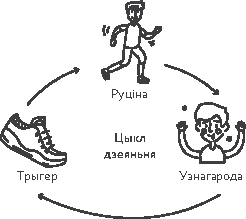
\includegraphics[scale=1.5]{willpower/ch14/8.pdf}
\end{figure}

Трэба дакладна ведаць, якую ўзнагароду дае вам звычка і як вы можаце атрымаць гэтую ўзнагароду іншым спосабам. Трэнінг замяшчэньня звычкі накіраваны на тое, каб вам дамагчыся падобнай узнагароды, выкарыстоўваючы іншае дзеяньне. Чым больш падобныя адчуваньні, тым больш эфэктыўная замена. Такім чынам, для зьмены звычкі вам трэба своечасова заўважыць дзеяньне трыгера, хваліць сябе, што вы змаглі гэта ўбачыць, і падтрымліваць жаданьне гэта заўважаць як мага часьцей. Затым вы сьвядома зьмяняеце дзеяньне на новае і атрымліваеце падобную з~ранейшай узнагароду ці фізычнае адчуваньне. Вы не змагаецеся супраць жаданьня нешта зрабіць, не прапануеце нешта іншае сабе, а~выкарыстоўваеце старую нэўронную схэму, замяніўшы ў~ёй адзін з~кампанэнтаў. Так мы можам пасьпяхова супрацьстаяць дэструктыўным імпульсам, накіроўваючы іх у~пазітыўнае рэчышча. Трэніруемся заўважаць трыгер і замяшчаць яго іншымі паводзінамі, якія вядуць да падобнага самаадчуваньня. Маем!

\subsection*{Пытаньні і заданьні}

1. Вызначыце выразныя трыгеры для сваіх звычак.

2. Прызначце сабе ўзнагароды (сьпіс) для падмацаваньня новай звычкі.

3. Якую шкодную звычку вы можаце замясьціць карыснай?


\section{Этап дзеяньня: актыўная праца над звычкай}

Мне вельмі падабаецца цытата палітыка Ўільяма X. Мюрэя: \emph{«Да таго часу, пакуль чалавек канчаткова на нешта ня вырашыцца, заўсёды застаюцца сумневы, магчымасьць адступіць, бязьдзейнасьць. Наконт любой праявы ініцыятывы існуе адна простая ісьціна, няведаньне якой забівае незьлічоныя задумы і вялікія ідэі: у~той момант, калі чалавек рашуча зьвязвае сябе абавязальніцтвамі, провід таксама пачынае дзейнічаць. У дапамогу гэтаму чалавеку здараецца мноства самых розных здарэньняў, якія інакш ніколі ня здарыліся б. Прынятае рашэньне цягне за сабой цэлы паток падзей: карысных супадзеньняў, сустрэч і прапаноў аб матэрыяльнай падтрымцы, у~якія ніхто і ніколі б не паверыў загадзя. Я адчуў глыбокую павагу да аднаго з~двухрадкоўяў Гётэ: ``Калі вы думаеце ці верыце, што на нешта здольныя, пачніце рабіць гэта. У дзеяньні~--- чараўніцтва, дабрадзейнасьць і сіла''».}

У пэрыяд разважаньняў і высьпяваньня варта і трэба сумнявацца і разважаць. Але калі ўжо надышоў прызначаны дзень, надышоў час штодзённай працы над звычкай. Нават калі ў~вас трэніроўкі два-тры разы на тыдзень, у~дні паміж імі таксама варта надаваць час звычцы~--- напрыклад, вывучыць тэхніку практыкаваньняў або прагуляцца 20 хвілінаў хуткім крокам. Калі мы штодня да нечага вяртаемся, імавернасьць доўгатэрміновай звычкі нашмат вышэйшая.

\textbf{Пэрыяд актыўнага дзеяньня} павінен складаць ня менш за 6--8 тыдняў ударных штодзённых намаганьняў. Гэта дапаможа замацаваць звычку ў~мозгу, успрымаць яе з~задавальненьнем, сфармаваць упэўненасьць і павысіць самаэфэктыўнасьць. Пры гэтым менш расказвайце пра звычку, больш рабіце. У гэты пэрыяд задача асвоіць навыкі важнейшая, чым нешта колькасна зьмяніць. Да канца этапу вы павінны лёгка ўмець рабіць тое, што хочаце разьвіць, супрацьстаяць спакусам і цалкам укараніць гэта ў~свой рэжым жыцьця, маючы трыгеры для запуску і ўзнагароды для замацаваньня посьпеху. Паступова само дзеяньне ўжо павінна стаць узнагародай.

Важна практыкаваць звычку ў~самых розных кантэкстах і сцэнарах, робячы ўсё большую колькасьць падыходаў ва ўсё большай колькасьці кантэкстаў. У ідэале вы павінны дасягнуць такога стану, каб сытуацыя не ўплывала на выкананьне прывычкі.

\textbf{Вы павінны лёгка выбягаць на вуліцу ў~мароз, дождж, туман, пасьля недасыпу, пасьля сваркі, у~поўню, у~зацьменьне~--- у~самых розных абставінах, каб пераадолець кантэкст-залежнасьць звычкі.}

Навучыцеся пераадольваць перапады жаданьня і энэргіі. Ня хочацца рабіць? Ну, зраблю і без задавальненьня, атрымаўшы ва ўзнагароду захаваньне ланцуга бесьперапынных дзеяньняў.

Магчыма, варта прадугледзець \textbf{незваротныя дзеяньні}~--- ``спаліць масты'',~--- калі вы нешта робіце аднаразова, і ўжо няма магчымасьці вярнуць гэта назад. Напрыклад, зьяжджаеце на пару месяцаў у~іншую краіну, каб вывучыць замежную мову, адклейваеце налепкі ад клавіятуры, каб асвоіць мэтад сьляпога друку. У іншых выпадках аддаяце тэлевізар, заводзіце сабаку, прадаяце машыну, плаціце за месяц дастаўкі хатняга харчаваньня і да т.~п.

Згодна з~прынцыпам маленькіх мэтаў, засяроджвайцеся на актыўным дзеяньні сёньня. Нагадваючы сабе, што ўчора і заўтра~--- гэта два дні, калі нічога не адбываецца, вы выкладаецеся сёньня, бо ``толькі сёньня мы можам зьмяніцца''. Розныя лічбавыя і папяровыя трэкеры са штодзённым адзначэньнем зробленага дапамагаюць вам ``не разрываць ланцуг''.

\begin{figure}[htb!]
  \centering
  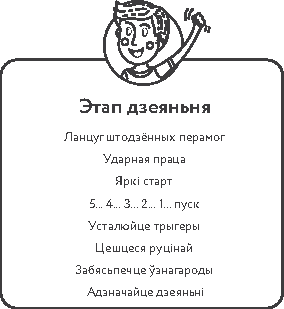
\includegraphics[scale=1.5]{willpower/ch14/9.pdf}
\end{figure}

\subsection*{Старайцеся}

Бяз вонкавага кантролю мы схільныя аслабляць дысцыпліну. Таму раз на тыдзень рабіце ўдарны дзень, паказваючы максімум з~таго, што можаце зрабіць: ідэальны рацыён, ідэальная трэніроўка, ідэальны занятак. Дык вы зможаце кінуць сабе выклік, задаць новыя стандарты і перасягнуць сябе. Не ўвязвайце ў~рутыне: кожны дзень пачынайце зь міні-перамогі ці рытуалу, які наладзіць вас на посьпех. На стадыі актыўнага дзеяньня важна надаваць адмысловую ўвагу падтрыманьню ўсьвядомленасьці, каб не сыходзіць у~скрайнасьці. З аднаго боку, не пераўзбуджаць і не выгараць, падтрымліваючы дастатковы ўзровень добрага стрэсу і алертнасьці, а~зь іншага~--- не заміраць у~сумневах і рэфлексіях.

\emph{Узгадайце міт пра Гаргону. Кожны, хто паглядзеў на мэдузу Горгону, скамянеў. Так і ў~кожнага чалавека ёсьць пытаньні ці думкі, якія прымушаюць яго сумнявацца ў~сабе і сэнсе таго, што ён робіць. Не вядзіце перамоваў са сваімі сумневамі, дзейнічайце! Проста не глядзіце на сваю мэдузу Гаргону!}

Ключавымі пагрозамі на стадыі звычкі зьяўляецца замена дзеяньня разважаньнем, самаабвінавачваньне (калі вы крытыкуеце, а~не падтрымліваеце сябе), ігнараваньне пагрозаў зрыву (захоўваеце дома цукеркі або алькаголь), неадэкватная ацэнка (ілюзіі посьпеху), заўчасныя паслабленьні, патураньні сваім жаданьням.

\textbf{Гераічны вобраз сябе.} Калі вы адчувае сумневы і няўпэўненасьць, то яны могуць паралізаваць ваша дзеяньне. Паспрабуйце адхіліцца ад іх, спытайце сябе, як бы гэта зрабіла ``лепшая версія вас''? Уявіце сабе яе, ``лепшую версію вас'', як калі б вы на 100\,\% рэалізавалі ўвесь свой патэнцыял, калі б у~вас былі неабмежаваныя магчымасьці для разьвіцьця сябе?

Таксама выкарыстоўвайце архетып героя для пераадоленьня супраціўленьня. Калі вам здаецца, што вы паўсядзённы са сваімі сумневамі, няўдалым досьведам, траўмамі ня зможаце зьмяніцца, то проста сыграйце ролю альтэр эга, у~якога ўсё атрымліваецца. Тэрмін альтэр эга ўвёў яшчэ Цыцэрон, вы таксама можаце прыдумаць сабе ``гераічную версію сябе''. Хто стане для вас такім вобразам? Гераічны вобраз дапаможа вам пакінуць непатрэбныя рысы за межамі сытуацыі і максымізаваць неабходныя. Вы як быццам актор, які выходзіць на сцэну, пакідаючы ў~зале сумневы і няўпэўненасьць. Сыграйце сваю ролю ідэальна, прыкідвайцеся тым, кім не зьяўляецеся, пакуль ня станеце ім. Галоўнае~--- гэта дзеяньне!

\textbf{Практыкуйце актыўнае процідзеяньне старым звычакам}, а~ня проста назірайце за імі. Нам цяжка рабіць дзьве розныя рэчы адначасова, таму перахапляйце ініцыятыву ў~вашых сумневаў і трывог. Пераключайце ўвагу, падтрымлівайце стымулюючы ўнутраны дыялог (я спраўлюся, я зраблю, я на правільным шляху), які інструктуе дыялог (прамаўляйце пра сябе пасьлядоўнасьць дзеяньняў, каб супрацьстаяць трывожным думкам). Актыўная рэляксацыя ці адцягненьне ад спакусы таксама добра дапамагаюць. Як толькі адчулі сумнеў, пачынайце адваротны адлік: «…5…4..3...2...1…старт»~--- і прыступайце да дзеяньня. Працуе цудоўна. Напрыклад, вы зьбіраецеся на трэніроўку і адчулі супраціў, пачынаеце адваротны адлік, хапаеце сумку і выскокваеце на лесьвічную пляцоўку. Усё!

\infobox{Памятайце: самае складанае ў~звычцы~--- гэта пачатак, ініцыяцыя дзеяньня патрабуе больш дафаміну, чым яе падтрыманьне. Як толькі вы пачалі, далей будзе нашмат лягчэй і цікавей.}

Часам могуць узьнікаць шкадаваньні аб страчаным камфорце. Мозг падкідвае ідэі, маўляў, можна і не асабліва імкнуцца, ты заслужыў гэта зьесьці, тут паляжаць, сюды патупіць… Сачыце бесстаронна за сабою: вы ўжо ведаеце кошт звычкі і гатовыя яе заплаціць, нягледзячы на нязручнасьці.

\textbf{Прынцып хваста яшчаркі} нагадвае: часта, каб выжыць, нам трэба ахвяраваць нават часткай сябе і свайго звыклага ладу жыцьця ў~абмен на магчымасьць жыць даўжэй і шчасьлівей. І гэта тая цана, якую мы гатовыя заплаціць. Каб захаваць жыцьцё, яшчарка адкідвае хвост, дзікі зьвер, які трапіў у~пастку, адгрызае сабе лапу,~--- няўжо мы ня можам адмовіцца ад малога, каб атрымаць нашмат больш?

\subsection*{Пытаньні і заданьні}

1. Штодня прытрымлівайцеся новай звычкі. Выкарыстоўвайце чэк-сьпісы, каб бачыць і адсочваць бесьперапынную мэту асваеньня звычкі.

2. Пазьбягайце залішніх сумневаў, акцэнтуйце ўвагу менавіта на дзеяньнях.

3. Выкарыстоўвайце зваротны адлік, каб хутка стартаваць.


\section{Этап утрыманьня звычкі: супрацьдзеяньне зрывам}

Ня так складана паспрабаваць нешта рабіць, складаней потым утрымлівацца. Таму пасьля «мядовага месяца» прапампоўкі звычкі мы павінны вучыцца яе захаваць.

\emph{Як заўважыў Арыстоталь: «Мы~--- тое, што робім пастаянна. Такім чынам, дасканаласьць~--- ня ўчынак, а~звычка».}

Як бы вы ні рыхтаваліся, як бы ні плянавалі, як бы ні былі матываваныя, зрывы і падзеньні для большасьці прадстаўнікоў роду чалавечага непазьбежныя. Сапраўдныя зьмены~--- гэта цяжка, бо вам даводзіцца ня проста выпрацоўваць новыя звычкі, але й сыходзіць з-пад улады старых.

\subsection*{Канструктыўна рэагуйце на зрыў}

Зрыў~--- гэта яшчэ не падзеньне, гэта папярэджаньне. Гэта нібы адмысловая шапаткая разьметка ля краю дарогі. Канструктыўная рэакцыя на зрыў~--- як пасьля націску трывожнай кнопкі~--- трэба распачаць праверку свайго пляна, знайсьці памылкі, улічыць іх і вярнуцца да зыходнага стану. Ёсьць вялікая колькасьць тыпавых сытуацый, дзе магчымы зрыў. Гэта зьмена ладу жыцьця (пераезд, зьмена працы і да т.~п.), узмацненьне нагрузкі (працоўны дэдлайн), зьмена кантэксту (развод), пагаршэньне здароўя (недасып, траўма, прастуда) і да т.~п. Больш за 70\,\% людзей пакідаюць шлях, сярэдні лік зрываў можа дасягаць 6--8, пакуль ня выпрацуецца доўгатэрміновая звычка.

\emph{Вы можаце загадзя сымуляваць магчымыя спакусы і зрывы, выпісаўшы ўсё, што можа зьбіць вас са шляху. Дождж і дрэннае надвор'е? Недасып? Прыступ трывогі? Як вы будзеце дзеяць у~такім стане? Чым большую колькасьць сытуацыяў вы змадэлюеце, тым устойлівейшымі да зрываў будзеце.}

\textbf{Хуткае вяртаньне.} Сам па сабе зрыў не небясьпечны, калі вы неадкладна вяртаецеся да выкананьня правілаў. Небясьпечней за ўсё, калі зрыў ператвараецца ў~рэцыдыў~--- поўнае вяртаньне да ранейшага. Кожная няўдалая спроба зьменаў небясьпечная тым, што падрывае веру ў~самаэфэктыўнасьць. Таму вельмі важна, каб памылкі не ператвараліся ў~падзеньне. Як гавораць у~народзе: страшна ня ўпасьці, страшна ня ўстаць пасьля гэтага. Ці гатовыя вы да падзеньня? Многія людзі любяць казаць аб тым, што яны будуць рабіць у~выпадку посьпеху, але баяцца нават думаць, што яны будуць рабіць у~выпадку правалу. Гэта нейкі страх «самазьдзейснага прароцтва», як быццам калі разглядаць нэгатыўныя сцэнары, то верагоднасьць іх павялічваецца. Важна выпрацаваць спакойнае стаўленьне да памылак, бо яны падказваюць вам, дзе ёсьць хібнасьці ў~вашых плянах і ў~ацэнцы.

\infobox{Памылкі~--- гэта навучаньне: ігнараваць свае памылкі, а~не вучыцца на іх,~--- гэта і ёсьць найвялікшая памылка.}

\textbf{Эфэкт ``к чорту ўсё!''.} Пры зрыве частай рэакцыяй бывае жага ўсё кінуць. Калі мы чакаем ад сябе ідэальных вынікаў, але не атрымліваем жаданага, то можам быць фрустраваныя. А каб пазбавіцца крыніцы фрустрацыі, гатовыя пахаваць свае спробы зьмяніцца. Унутраны дыялёг правакуе зрыў: ``Адзін раз ня страшна, ты заслужыў, сёньня сьвята, не пазбаўляй сябе гэтага, жывём толькі раз''. Замест пэрфэкцыянізму і самакрытыкі праявіце да сябе спачуваньне, нагадайце, што памыляюцца ўсе, і зараз трэба апэратыўна вяртацца ў~выбраную каляіну.

\begin{figure}[htb!]
  \centering
  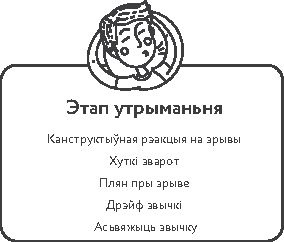
\includegraphics[scale=1.5]{willpower/ch14/10.pdf}
\end{figure}

\textbf{У момант спакусы} дапамагае проста зрабіць паўзу, не рабіць ніякіх дзеяньняў, спыніцца. Дыхайце (можна па праграме ў~тэлефоне), вазьміце падтрымку (патэлефануйце вашаму мэнтару ці сябру), адцягніцеся (зрабіце тое, што цалкам паглынае ўвагу: тэтрыс, планка, пазл, відэагульня, складаная кніга, хуткая хада), пакіньце месца дзеяньня трыгера, уключыце процідзеяньне (замест разважаньняў аб гэтым эклеры прачытайце яшчэ раз вашу мэту і матывацыю), успомніце досьвед пасьпяховага пераадоленьня такой жа праблемы ў~мінулым. Пасьля таго, як хваля спакусы спадзе, прааналізуйце: чаму вы так сябе паводзілі, што спрацавала? Чаму трыгер быў такі моцны?

\emph{Важна разумець, што дафамінавая прырода апанавалага жаданьня пры эфэкце «к чорту ўсё» мае кароткі прамежак дзеяньня. Напрыклад, вы не ясьце салодкага і вырашылі патрэніраваць волю. Бяз грошай і карты ідзяце ў~кавярню, выбіраеце свой любімы эклер і гледзіце на яго, уважліва назіраючы за тым, што адбываецца ў~вас усярэдзіне.}

\emph{Хваля жаданьня, якая ахоплівае вас, здаецца такой моцнай, што ёй прасьцей падпарадкавацца, пакуль яна вас не разарвала. Выступае пот, слабеюць калені. Яшчэ сэкунда, і ўсё~--- дафамінавы сыгнал па мэханізьме зваротнай сувязі блакуе сам сябе. Вы са зьдзіўленьнем аглядаецеся, нават бянтэжачыся таго, якія эмоцыі ў~вас мог выклікаць гэты кавалак цеста з~тлушчам. Такі сэрфінг спакусаў дапаможа вам зразумець, што імпульсы «ўсё кінуць» кароткатэрміновыя, і іх досыць лёгка вытрымаць. Не супраціўляйцеся эмоцыям, дазвольце ім прайсьці праз вас і растаць. Пры гэтым, зразумела, вытрымліваючы вонкавы кантроль.}

\textbf{Пан або прапаў.} Вельмі часта ў~стрэсе, у~стоме, калі высільваецца прэфрантальная кара, наша мысьленьне становіцца чорна-белым: ці поўная перамога, ці канчатковы пройгрыш. Калі зьяўляюцца думкі аб сваёй няздольнасьці зьмяніцца, прытрымлівацца новай звычкі або пазьбегнуць старой, то вера ў~самаэфэктыўнасьць падае, і мы глядзім у~будучыню пэсімістычна.

\emph{«Калі з~прычыны абставінаў парушаецца раўнавага духу, аднаві самавалоданьне як мага хутчэй і не заставайся ў~прыгнечаным настроі занадта доўга, інакш табе ўжо нічым нельга будзе дапамагчы. Звычка аднаўляць гармонію ўдасканаліць цябе»,~--- рымскі імпэратар, філёзаф Марк Аўрэлій.}

У такі момант важна выкарыстоўваць навык усьвядомленасьці і не рэагаваць на стрэсавыя думкі~--- яны сыдуць, як толькі наш фізычны стан зьменіцца. Нагадайце сабе, што памылкі~--- гэта частка працэсу навучаньня, і цяпер важна не перажываць, а~вярнуцца ў~норму. Вы проста пасьлізнуліся~--- так бывае. Пахваліце сябе, калі пасьпяхова пераадолееце зрыў.

\subsection*{Плян пры зрыве}

Калі вы ў~стане стрэсу, то прыдумаць нешта добрае цяжка. Трэба мець плян Б: як вы вернецеся да мэты ў~выпадку зрыву? Пра што вы зараз можаце думаць (процідзеяньне звычкі) і ня думаць (сумнявацца ў~сабе), якія дзеяньні вам вернуць упэўненасьць, як вы можаце паклапаціцца пра сябе, а~што катэгарычна нельга рабіць, да каго вы можаце зьвярнуцца па падтрымку? Якое дзеяньне вы можаце зрабіць проста зараз, каб узяць сытуацыю пад кантроль і падтрымаць рух да мэты? Ваш плян павінен уключаць мерапрыемствы на сёньняшні і заўтрашні дзень, а~таксама дакладна сфармуляваную мэту і матывацыю вашай зьмены. Насіце яго з~сабой у~тэлефоне або раздрукаваным на паперы.

У выпадку высокай нагрузкі, калі вам бракуе энэргіі і сіл выконваць звычку ў~поўным аб'ёме, варта мець ``аблегчаны плян'', які дапаможа захаваць звычку і не запатрабуе ад вас залішніх валявых намаганьняў. І важна выканаць гэтае маленькае дзеяньне, каб не разарваць штодзённы ланцуг фармаваньня звычкі.

\textbf{Трыгеры высокай рызыкі}~--- гэта людзі, абстаноўка, словы, дзеяньні, эмоцыі, якія асацыююцца зь непажаданымі паводзінамі і выклікаюць моцнае жаданьне да яго вярнуцца. Напрыклад, калі вы выпівалі зь сябрамі, то сустрэча зь імі можа выклікаць такое жаданьне. Большасьць раньніх зрываў выкліканая менавіта старымі трыгерамі. Пры гэтым дзеяньне трыгера неўсьвядомленае, мозг рацыяналізуе і прыдумляе фармальна лягічныя нагоды, падставы і зачэпкі для вяртаньня да старой звычкі. Такімі чыньнікамі можа стаць усё, што зьніжае кантроль і ўсьвядомленасьць: стрэс, моцныя станоўчыя і адмоўныя эмоцыі, сацыяльны ціск, канфлікт, фізычная і псыхалягічная цяга.

Назіраючы за сабой, выявіце асабістыя трыгеры высокай рызыкі. Запішыце, дзе і калі ў~вас узьнікае жаданьне сарвацца? Хто пры гэтым прысутнічае побач? Пра што вы думаеце, што адчуваеце і што робіце?

\infobox{Як правіла, 20\,\% трыгераў адказваюць за 80\,\% зрываў: выявіўшы самыя галоўныя, вы зможаце павысіць сваю эфэктыўнасьць. Галоўнае~--- не прапускаць трэніроўкі, не заядаць, не прапускаць раньні ўздым два разы запар.}

На самым раньнім этапе фармаваньня звычкі важна пазьбягаць трыгераў. Але бясконца гэта рабіць ня варта, бо пазьбяганьне можа прывесьці да інкубацыі і ўзмацненьня іх дзеяньня. Па меры павышэньня сілаў і веры ў~сябе трэба пераходзіць да экспазіцыйнай тэрапіі: падвяргаць сябе кароткатэрміноваму ўзьдзеяньню трыгераў, пасьпяхова пераадольваючы іх узьдзеяньне. Важнай умовай захаваньня звычкі будзе ўмацаваньне асабістых межаў: навучыцеся адмаўляць, ветліва казаць ``не'' безь зьбянтэжанасьці, страху крыўды або боязі падацца грубіянам.

\subsection*{Пытаньні і заданьні}

1. Ці часта вы зрываецеся, калі асвойваеце звычкі? Як хутка вяртаецеся да іх?

2. Якія трыгеры мацней за ўсё правакуюць вас? Складзіце падрабязны сьпіс.

3. Складзіце плян дзеяньняў у~выпадку зрыву.


\section{Кантроль над асяродзьдзем}

Асяродзьдзе ўплывае на нашы паводзіны мноствам усьведамляльных і неўсьвядомленых спосабаў. Прыклады такога ўплыву мы ўжо разглядалі ў~папярэдніх разьдзелах. Напрыклад, малюнак вачэй прымушае нас паводзіцца больш адказна і прасацыяльна, а~тэлефон, які ляжыць побач, зьніжае нашы кагнітыўныя здольнасьці. 

\textbf{Мы ствараем асяродзьдзе, а~асяродзьдзе стварае нас, уплываючы на нашы звычкі.} Падумайце, што ў~навакольным асяродзьдзі дапамагае, а~што перашкаджае ў~фармаваньні вашай звычкі? Мы можам стварыць асяродзьдзе, якое будзе нас падштурхоўваць займацца спортам, класьціся своечасова спаць ці добра харчавацца. Мы можам зьнізіць рызыку зрыву, калі прыбяром рэчы, якія нагадваюць аб праблеме, і будзем пазьбягаць людзей, якія яе правакуюць.

\emph{Мы можам кіраваць сваёй фізыялоёіяй з~дапамогай навакольных прадметаў. Напрыклад, выкарыстоўваць меншыя па памеры лыжкі і талеркі, кубкі з~тоўстым дном, цяжкі посуд~--- гэта аўтаматычна зьнізіць колькасьць зьяданай ежы. Калі мы будзем есьці строга на кухні, засьцілаючы стол абрусам, то неўзабаве жаданьне перакусіць у~кабінеце аслабне і зьнікне.}

\infobox{Каб не змагацца са спакусай пасэрфіць у~інтэрнэце падчас працы, вы можаце выкарыстоўваць розныя прыборы для рознага тыпу працы: напрыклад, сэрфіць толькі на смартфоне, а~ноўтбук выкарыстоўваць адно для працы.}

Кожная звычка існуе ў~нас у~мозгу не сама па сабе, а~\textbf{прывязаная да пэўнага кантэксту}, у~якім яна сфармавалася і ў~якім мы яе выкарыстоўваем. Само паняцьце “кантэкст” адносіцца да ўсяго, што нас атачае: рэчы, людзі, час, месца. Часта кантэкст, насычаны старымі сыгналамі, зьяўляецца перашкодай на шляху да зьменаў. Напрыклад, вы некалькі разоў перакусілі печывам на працоўным стале~--- і ўсё, зараз мозг будзе вам пэрыядычна, асабліва ў~стрэсе, падкідваць жаданьне зьесьці печыва, калі вы працуеце. Ці вы прывыклі хадзіць у~адну спартыўную залу да канкрэтнага трэнера, а~ён сышоў~--- і ўсё, вы перасталі трэніравацца. 

\textbf{Добрым прыкладам кантэксту можа быць сэрвіроўка стала: заслалі абрус~--- і паелі, потым прыбралі. Няма абруса~--- і няма чаго глядзець на ежу.} 

Таму варыянтам для зьмены звычак можа быць пераезд у~іншае месца, дзе кантэкст настолькі новы, што старых трыгераў там папросту няма фізычна. У новым месцы лягчэй схуднець, лягчэй завязаць зь любой залежнасьцю. Нашы звычкі, у~ісьце сваёй, шаблоны, у~аснове якіх ляжыць сыгнал і адказ на яго: зьнікне сыгнал~--- зьнікне і адказ. Зьмена кантэксту можа дапамагчы прыслабіць дзеяньне як нэгатыўнага, так і пазітыўнага асяродзьдзя, таму пераезд ня толькі дасьць магчымасьць пазбавіцца шкодных звычак, але й здольны прывесьці да зьнікненьня добрых звычак. Правярайце сябе, каб ня страціць важнае! 

\textbf{Ня псуйце сваю рутыну.} Адступленьні ад правілаў можна дазволіць сабе толькі ў~іншым кантэксьце. Хай сяброўскія вячоркі ``зь віном'' будуць у~кавярні ў~далёкай частцы горада, а~не на вашай кухні. Пакіньце дом і працоўнае месца прасторай чыстае рутыны.

\emph{Неяк пасьля пераезду мы парушылі гэтае правіла, і жонка потым сьмяялася: «Усё, сапсавалі новую кватэру~--- цяпер толькі прадаваць».}

\subsection*{Пытаньні і заданьні}

1. Ці падзяляеце вы працу і адпачынак?

2. Які кантэкст дапамагае вам прытрымлівацца сваіх звычак?

3. Як зьмяніць асяродзьдзе, каб яно падтрымлівала вас?


\section{Доўгатэрміновае падтрыманьне зьменаў}

Чым даўжэй мы практыкуем звычку, тым імаверней, што яна застанецца з~намі надоўга. У цэлым розным людзям можа спатрэбіцца ад 60 да 200 дзён, каб звычка замацавалася. Але нават шматгадовыя звычкі могуць быць крохкімі. Цяжкі стрэс здольны выклікаць псыхалягічны рэгрэс, а~зьмена абставінаў прывесьці да страты звычкі. 

\emph{Мы можам страціць звычку, калі зьнік трыгер, абясцэнілася ўзнагарода, зьмяніўся кантэкст.}

Мы можам лічыць звычку замацаванай, калі яна аўтаматызаваная. Гэта значыць~--- адсутнічае момант прыняцьця рашэньняў аб пачатку дзеяньня, аб самім дзеяньні, аб узнагародзе. Мы проста дзейнічаем, і розум пры гэтым вольны. Звычка становіцца навыкам, нэўронным ланцужком, мы робім яе лёгка і без прымусу, яна добра ў~нас атрымліваецца, мы хочам яе рабіць, атрымліваем ад яе задавальненьне і карысьць адначасова.

\infobox{Аптымальна, калі мы прадчуваем магчымасьць заняцца гэтай справай, калі сама магчымасьць практыкаваць звычку зьяўляецца ўзнагародай, калі звычка прыносіць больш задавальненьня, энэргіі, часу, чым патрабуе для выкананьня.}

У доўгатэрміновай пэрспэктыве звычка становіцца часткай нашага ладу жыцьця, мы ідэнтыфікуемся зь ёю, не ўяўляючы свайго жыцьця безь яе. Мы дзівімся: «Не магу ўявіць, як я раней жыў бяз гэтага». Тут ужо вонкавая матывацыя перайшла ва ўнутраную.

\textbf{Эфэкт фінішнай рысы.} Адна з~ключавых пагроз доўгатэрміновым звычкам~--- гэта «парадокс пераможцы». Калі вы дасягнулі мэты, мозг лічыць справу завершанай і зьніжае матывацыю. Вам здаецца, што можна расслабіцца, бо вы перамаглі. Таму важна сфармуляваць сваю мэту так, каб яна не сабатавала вас.

\emph{На жаль, часовы посьпех не гарантуе доўгатэрміновага. Так, 70\,\% маці, якія кінулі курыць падчас цяжарнасьці, пачынаюць пасьля завяршэньня груднога гадаваньня. Схуднелыя да лета, увосень і ўзімку набіраюць яшчэ больш лішніх кіляграмаў. Так дасягненьне мэты зьяўляецца пачаткам зрыву!}

\textbf{Дрэйф звычкі.} Дрэйф звычкі~--- гэта паступовае, павольнае яе згасаньне, якое мы можам нават не заўважаць. Мы пачынаем рабіць больш ``выключэньняў'', нашы паказьнікі пагаршаюцца, узнагароды прыядаюцца. Агульнае зьнясіленьне прыводзіць да таго, што мозг пачынае ``эканоміць'', і найболей пэрспэктыўныя звычкі зьлятаюць першымі. Калі навакольнае асяродзьдзе застаецца таксічным, супраціўляецца зьменам, патрабуе кампрамісаў з~тым, што мы лічым правільным, то мы неўпрыкмет для сябе можам падпарадкавацца сацыяльнаму ціску.

\textbf{Самападман}~--- гэта мэханізм, калі мы апускаем планку і свае ўнутраныя стандарты, апраўдваючы гэта рознымі спосабамі. Многія людзі пачынаюць прыдумляць адгаворкі і розныя ``асаблівыя абставіны''. Яны адчуваюць «ілюзію бязгрэшнасьці», пагарду да маніторынгу, інструкцыі, кантролю, а~замест гэтага ў~іх зьяўляецца нейкая вера, што яны і так усё добра робяць і дадуць рады самі.

\emph{Напрыклад, лекары зь вялікім досьведам могуць рабіць нават больш памылак, чым пачаткоўцы. Такія людзі супакойваюць сябе фразай ``прынамсі я лепшы, чым…''.}

\textbf{Пастаянны аб'ектыўны маніторынг} свайго прагрэсу абавязковы. Без вымярэньня ня можа быць руху наперад. Наш мозг гатовы прыдумаць сотні апраўданьняў і фальшывых прычынна-выніковых сувязяў, каб апраўдаць што заўгодна. 

\infobox{Важна адсочваць вынікі, не дапускаючы іх паніжэньня. Так, вы ня зможаце рабіць ідэальна, але можна ў~будучыні стаць лепшымі, чым былі, перасягнуць сябе!}

Існуюць розныя шчылінкі розуму, якія важна ведаць і не трапляцца: ``Ем, таму што няшчасны, а~няшчасны, таму што тоўсты'', можна ``заслужыць патураньне'', ``сёньня адпачываю, усё буду рабіць заўтра'', ``празьмернасьці сёньня забясьпечаць лепшы самакантроль заўтра''~--- маўляў, можна зь лішкам наесьціся, найграцца так, што потым і не захочацца. Розум можа падманваць нас кагнітыўным скажэньнем фальшывых альтэрнатыў, напрыклад, я аб'ядаюся ў~фастфудзе, затое зь сябрамі, або чэзну над салатай дома ў~адзіноце; я не магу трэніравацца, таму што шмат працую. Скептычна стаўцеся да такіх думак: вы можаце і працаваць, і трэніравацца,~--- трэніроўкі толькі палепшаць вашу прадуктыўнасьць. І малаверагодна, што сумеснае абжорства~--- гэта найлепшы спосаб умацаваньня сацыяльных сувязяў.

Часам людзі перакладаюць адказнасьць на вонкавы кантроль, абвінавачваючы паездкі, траўмы, надвор'е, дзяцей, сьвяты, самаадчуваньне, чыноўнікаў, бацькоў. Неўсьвядомлена людзі могуць прадпрымаць ``арганізаваныя няўдачы''~--- загадзя неадэкватныя дзеяньні, якія вядуць да зрыву. Напрыклад, рэзка перайсьці з~булак на сырую зеляніну, гародніну і бабовыя, а~потым пакутаваць метэарызмам і ў~выніку абвясьціць, што ``здаровае харчаваньне~--- сапраўды не для мяне''. Або сарваць сьпіну на трэніроўках з~дрэннай тэхнікай і суцяшаць сябе, што і сілавы спорт зусім не маё .

Або вось бясконцыя адкладаньні: напрыклад, ``не пачну працаваць над кнігай, пакуль ня вырастуць дзеці'', ``ня буду есьці правільна, пакуль не куплю тую кнігу з~рэцэптамі''. Яшчэ сустракаецца псэўдатурбота пра іншых: «я не раблю нешта і не хачу мяняцца, каб сацыяльна ўпісацца і ``не траўмаваць'' навакольных сваёй дасканаласьцю». Часам людзі трапляюць у~пастку фальшывай самаактуалізацыі: ``жывём адзін раз, таму ня трэба адмаўляцца ад цукру, алькаголю, порна, я такі, які ёсьць'',~--- як апраўданьне сваіх шкодных звычак.

\subsection*{Асьвяжыць звычку}

Гавораць, навічкам шанцуе: навізна сапраўды робіць усё больш прыцягальным, але чым больш праходзіць часу, тым больш нуднымі могуць станавіцца звычкі. Таму важна іх асьвяжаць, перазапускаць у~новым фармаце. Так мы можам узламаць рутыну, знайсьці новае натхненьне, падтрымліваць адчуваньне росту і трансфармацыі. Звычку можна асьвяжыць, калі посьпехі затрымаліся на плато ці пасьля значных зьменаў у~жыцьці: шлюб, зьмена месца жыхарства, працы і да т.~п. Асьвяжыць звычку дапамогуць ударныя заняткі, удзел у~маратонах, спэцыяльныя трэніроўкі асобных аспэктаў навыку, практыка ў~новых умовах і ў~новым сацыяльным асяродзьдзі.

Пэрыядычна плянуйце такія перазапускі з~чыстага аркуша, вяртаючыся да сваіх першых запісаў плюсаў і мінусаў, матывацыі, абавязацельстваў. Вылучыце сабе дзень на тыдзень, калі вы ўзорна будзеце прытрымлівацца сваіх звычак, робячы «ідэальны дзень».

\textbf{Партызанскі ЗЛЖ}, або Як займацца здароўем, не прыцягваючы ўвагі. Многія людзі скардзяцца, што калі яны пачынаюць больш інтэнсіўна займацца сваім здароўем, то ў~іх узьнікаюць непаразуменьні і канфлікты з~навакольнымі людзьмі. Маўляў, я хачу як лепш, а~гэтыя няўдзячныя яшчэ раздражняюцца! Так, вашыя зьмены могуць нашкодзіць сацыяльнай адаптацыі і справакаваць адыходжаньне ад звычак. Давайце разьбяромся, чаму ўзьнікаюць такія сытуацыі.

\textbf{Уварваньне ў~асабістыя межы.} Няпрошаная парада~--- гэта ўварваньне ў~межы. Той, хто раіць, павышае свой статус, а~статус таго, каму даюць парады, зьніжаецца. Нікому не падабаецца, калі нехта спрабуе зьніжаць яго статус, таму такія парады (нават магчыма карысныя) толькі раздражняюць і выклікаюць абурэньне. Ня ўмешвайцеся, калі вас не пытаюцца ці вашыя парады не зьвязаныя з~тэмай размовы.

\textbf{Самасьцьвярджэньне.} Вы спрабуеце падняць сваю самаацэнку за кошт іншых людзей. Вы ясьце, бегаеце ``правільна'', таму вы добры і правільны. Той, хто ня робіць гэтага, -- ``няправільны''. Асуджаючы іншых людзей, крытыкуючы або пазьбягаючы іх, вы павышаеце сваю самаацэнку. Напрыклад, у~артарэксіка самаацэнка цесна завязаная на тым, што ў~ягонай талерцы. Ацэньваць людзей па іх талерцы~--- бязглузда; няправільна падымаць самаацэнку за кошт іншых.

\textbf{Шкода парады.} Часта погляды і звычкі чалавека зьяўляюцца часткай яго самаідэнтыфікацыі. І крытыку ягонага ладу жыцьця ён успрымае як асабістыя нападкі. Таму вашыя парады яшчэ мацней пераконваюць яго ў~слушнасьці сваіх поглядаў і ў~памылковасьці вашых.

\textbf{Зьніжэньне матывацыі.} Калі вы ўвесь час дзеліцеся сваімі плянамі, гэта парадаксальна можа зьмяншаць матывацыю. Вы «спажываеце будучыню», мозг успрымае задачу ўжо як выкананую. Акрамя таго, гэта можа выклікаць скепсіс і крытыку вашых плянаў з~боку таксічных людзей. Дзяліцеся плянамі толькі з~тымі, хто безумоўна вас падтрымлівае, і ў~пляне падтрымкі і коўчынгу, а~не фантазіяў.

Што рабіць? Не навязвайце свае погляды. Будзьце тактоўнымі, каб іншыя людзі пачуваліся камфортна побач з~вамі, пазьбягайце прамых сутыкненьняў і ўмейце адыходзіць ад спрэчак. Напрыклад, ня варта за агульным сталом публічна заяўляць, што вы не ясьце салодкае, калі імяніньнік рэжа торт. Пакладзяце кавалачак за талерку або паспрабуйце загарнуць. Калі вакол вас усё з~келіхамі шампанскага, ня варта чытаць публічныя лекцыі пра шкоду алькаголю. Наліце вады ў~келіх і будзьце на адной хвалі. Вядома, расказвайце пра свае здаровыя звычкі тым, каму гэта сапраўды цікава, і адсякайце троляў. А ў~іх узьнікаюць пытаньні да вашай талеркі, то ня трэба чытаць лекцыю пра глікемічную нагрузку, прадумайце шляхі адыходу (ня п'ю, бо на антыбіётыках, алергія на цукар, доктар забараніў і да т.~п.). Не кажыце пра тое, што робіце, калі вас пра гэта не пытаюцца і ня просяць парады.

\subsection*{Пытаньні і заданьні}

1. Ці падае якасьць выкананьня і строгасьць вашых старых звычак зь цягам часу?

2. Як зрабіць старую звычку цікавейшай? Складзіце сьпіс ідэй. Якую вобласьць вашага жыцьця вы хочаце абнуліць і пачаць нанова?

3. Як навакольныя замінаюць вашым здаровым звычкам?

\clearpage
\thispagestyle{empty}
\begin{figure*}[htb!]
  \vspace*{-0.5in}
  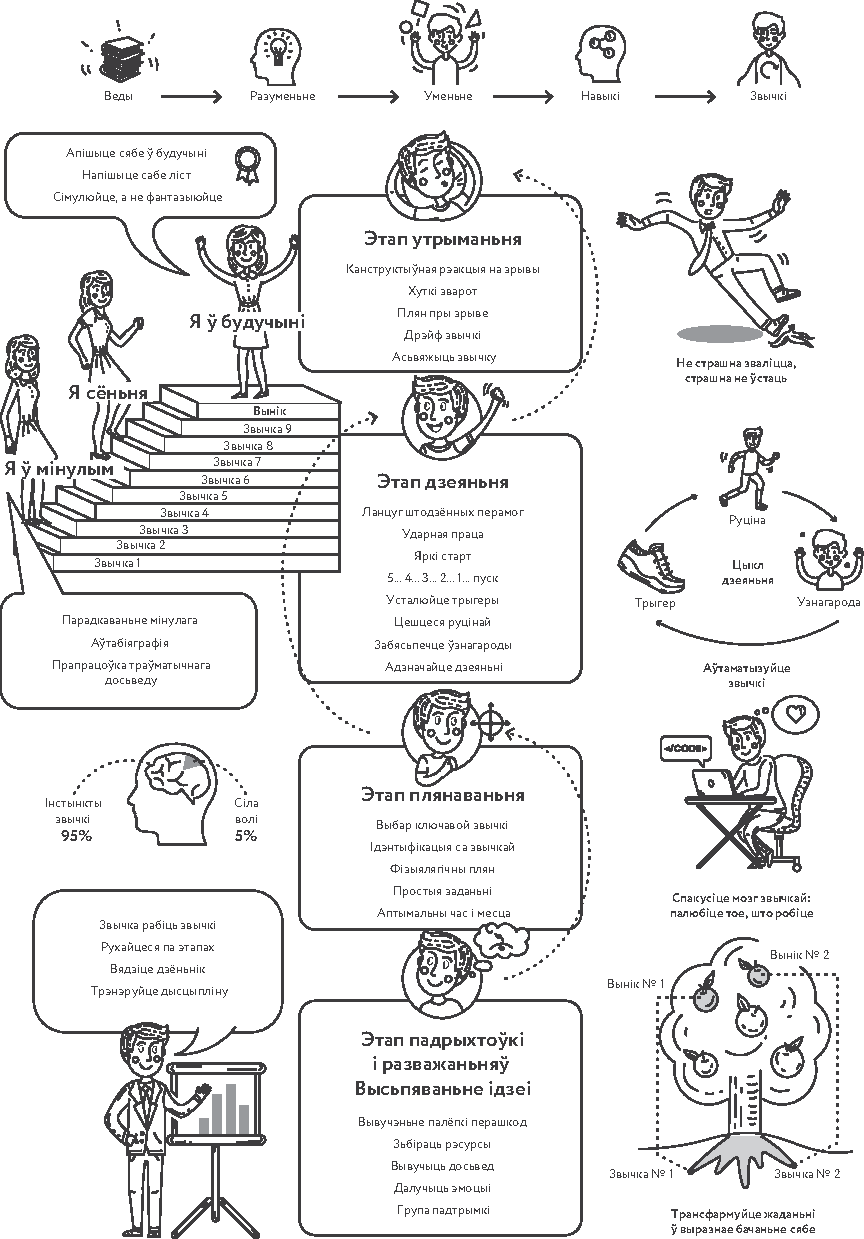
\includegraphics[width=\textwidth]{willpower/ch14/full.pdf}  
\end{figure*}
